\chapter{Analyse der jetzigen Situation der Pirelli Deutschland GbmH}
\label{cha:analyse}

\section{Situationsbeschreibung}
\label{sec:situation}

Die bestehende Situation der PD spielt für die spätere Umsetzung eine große Rolle und muss somit im Näheren betrachtet werden.
Zu Beginn des Projektes wurden bereits diverse Systeme zur Überwachung des Netzwerkes eingesetzt.
Die Überwachung des Netzwerks lässt sich bei näherer Betrachtung in folgende Punkte unterteilen:\\
\\
Darstellung und Überwachung des Netzwerkequipments\\
Überwachung von Diensten/Servern\\
Überwachung des Netzwerkverkehrs\\
Überwachung von einzelnen Hosts im Netzwerk\\

Zur Überwachung der Stati der einzelnen Netzwerkgeräte, im Speziellen die Switches und Router, wird das Programm “OpenView Network Node Manager” von HP verwendet.
Zurzeit wird das Programm verwendet, um eine automatische Übersicht über die Relationen zwischen den Switches und Routern und eine grafische Übersicht über den Status der Switchs und Router zu erhalten.
Über dieses Programm können auch Server und deren Dienste erfasst werden.
Diese Funktion wird jedoch aktuell nicht mehr mit Daten gepflegt, da hier aktuell ein Transfer zum Nagios System stattfindet. Der Transfer findet aufgrund der Tatsache, dass die Wartung von OpenView ausgelaufen ist, statt.\\\\
Für die Überwachung spezieller Hosts (in der Praxis meist Server) und Diensten, kommt das Open Source System Nagios zum Einsatz, welches ein hohes Maß an Flexibilität und Modularität bietet.
Dieses Programm ermöglicht es, diverse Dienste im Netzwerk auf vorgegebenen Hosts abzufragen und diese anschließend zu visualisieren.
Zusätzlich können verschiedene Warn- und Fehlerlevels für einen Service definiert werden, die im Falle einer Störung Warnungen an vordefinierte Personen verschicken.
Dieses System ist somit hauptsächlich für die Überwachung der Dienste zuständig.\\\\
Zur Untersuchung von Netzwerk-Traffic zwischen verschiedenen Netzwerken kommt das System MRTG zum Einsatz, welches hauptsächlich für das Anzeigen des Netzwerktraffics auf Routern ausgelegt ist.
Dieses wird im Unternehmen hauptsächlich zum Erfassen der Bandbreitennutzung der Router bzw. der WAN-Verbindungen verwendet.
Dies ist vor allem wichtig, um den aktuellen Traffic zwischen den einzelnen Standorten in Deutschland im Überblick zu behalten.\\\\
Abschließend gibt es noch ein System von Cisco mit dem Namen “CiscoWorks”, welches dazu dient, mit einem speziellen Programmteil die Hosts an den jeweiligen Switches zu erkennen und zu identifizieren.
Hier werden nicht nur simple Zuordnungen zwischen MAC-Adresse des Hosts und des Switches, bzw. des Port des Switches hergestellt,
sondern umfangreiche Informationen gesammelt, z.B. über die Geschwindigkeit des Anschlusses, die IP und der DNS-Hostname des Gerätes.
Hinzu kommen Details, wie der Gerätetyp, welcher einem die Möglichkeit gibt, zu erkennen, ob es sich hierbei um ein Switch oder Router handelt.\\
Da es bei diesem System notwendig ist, regelmäßig die Lizenz zu verlängern, um auch weiterhin die neusten Router und Switches zu unterstützen, ist hier eine gewisse Abhängigkeit gegeben.
Weil von CiscoWorks selbst nur ein kleiner Teil genutzt wird und somit die Lizenzkosten unverhältnismäßig zur Nutzung sind, wurde entschieden, dieses in Zukunft zu ersetzen.\\\\
Neben der eingesetzten Software, ist es auch wichtig ein Überblick über die Netzwerk-Architektur zu haben.
Auf diese wird im nachfolgenden Abschnitt eingegangen.
Das Netzwerk bei PD ist in verschiedenen Hierarchieebenen konzipiert.
In der untersten Ebene stehen die Switches an denen die Hosts angeschlossen sind. Diese Ebene wird als Access-Layer bezeichnet.
Über dieser Ebene wiederrum befindet sich der Distribution-Layer. In diesem sind Switches zu finden, welche alle Access-Layer Switches verbinden und als Schnittstelle zu den Layer 3 Switches, den sogenannten Core-Switches, dienen.
Die Core-Switches können zusätzlich anhand von OSI-Layer-3 Informationen Forwarding betreiben.
Die komplette Anordnung ist in Abbildung \ref{fig:network_ex1} zu sehen.

\begin{figure}[H]
\centering
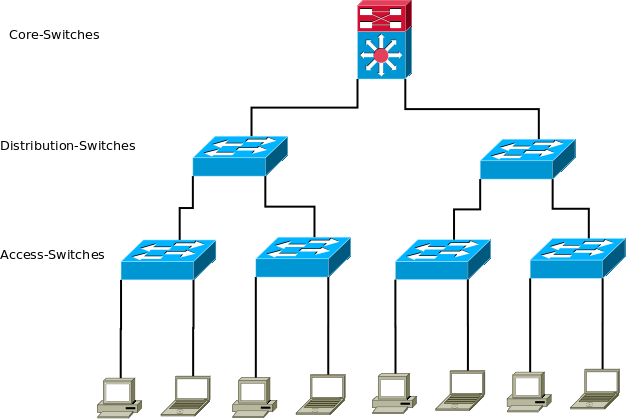
\includegraphics[width=0.9\textwidth]{network_ex1.png}
\caption{Netzwerkarchitektur PD}
\label{fig:network_ex1}
\end{figure}

\section{Anforderungsdefinition}
\label{sec:anfdef}

Um das bestehende System ersetzen zu können, muss zunächst untersucht werden, welche der bereits vorhandenen Funktionen im aktuell verwendeten System genutzt werden und welche in Zukunft benötigt werden.
Im Anschluss an diese Untersuchung müssen auch weitere potentielle Aufgaben berücksichtigt werden, um eine Erweiterbarkeit des Systems zu garantieren.
Damit das neue System allen Anforderungen gerecht wird, empfiehlt es sich zunächst, sich mit den Personen zusammen zu setzen, die das bestehende Programm zurzeit nutzen.\\
Hierbei wird nicht nur auf die aktuelle Nutzung eingegangen, sondern auch diese kritisch hinterfragt, ob eventuelle Anforderungen bereits von anderen Systemen erfüllt werden.
Durch Gespräche mit den zuständigen Mitarbeitern wurden diverse Anforderungen erörtert.\\\\
Als wichtigster Punkt ist die Erkennung der Hosts, sowie der zugehörigen Ports an den Switches zu sehen.
Diese ist notwendig um den Ort eines Hosts im Netzwerk festzustellen. Praktische Anwendung hat dies, wenn zum Beispiel ein Host aufgefunden werden muss, wenn der zugehörige Mietschein des Computers ausläuft und dieser zurückgegeben werden muss.
Hier ist es nicht selten der Fall, dass der Computer mit seinem dazugehörigen Besitzer bereits die damalige Abteilung verlassen hat und dieser somit nicht mehr auffindbar ist.
Eine weiterere Anwendungsmöglichkeit ist, dass der Helpdesk wissen möchte, wenn es Probleme mit einem Computer gibt, ob die Netzwerk-Hardware bis zum Host einwandfrei funktioniert. Hierfür muss man nicht nur wissen, an welchem Ort der Host sich befindet, sondern auch die dazugehörigen Ports.
Da die Ports als auch die Switches ausgelesen werden, kann man somit zeitnah eine Rückmeldung geben, dass der Switch, sowie dessen Port einwandfrei funktionieren, oder falls dies nicht der Fall ist, den Fehler besser lokalisieren. Somit ist selbst bei keinerlei Kenntnis des Hosts außer der DNS oder der IP, eine direkte Lokalisierung und Bewertung des Status möglich.\\\\
Ein weiterer wichtiger Aspekt ist die Möglichkeit genau herauszufinden, welche Hosts hinter einem Port angeschlossen sind.
In der Praxis ist dies wichtig, da es vorkommen kann, dass unerwünschte Netzwerkgeräte angeschlossen wurden.
Normalerweise befinden sich im Unternehmen an einem Port eines Switches der untersten Ebene maximal zwei Hosts. Der Großteil der Ports hat nur einen Host zum Beispiel den Computer eines Mitarbeiters oder ein Netzwerkgerät.
In einem Teil der Fälle ist dieser Computer nicht direkt an den Port des Switches angeschlossen, sondern wird über den Port eines VOIP-Telefons durchgeschleift, welches dann an den Switch angeschossen ist.
In diesem Fall sind auf dem Port zwei Hosts zu sehen.
Dies ist der Soll Zustand. Jedoch kann es vorkommen, das Mitarbeiter im Werk ohne Erlaubnis fremde Netzwerkgeräte anbringen, sei es ein Hub, ein eigener WLAN-Router oder andere Geräte. Da diese Geräte die Sicherheit des Netzwerkes beeinflussen, müssen diese identifiziert und gleichzeitig lokalisiert werden können um eine Entfernung zu ermöglichen.
Hinzu kommt der Punkt einer möglichen Historie, wann welcher Host an welchem Port bzw. Switch angeschlossen war. Hierbei soll erkennbar sein, an welchem Port der Host war, jedoch ist es nicht notwendig zu wissen wie oft dieser dort angeschlossen war.
Daraus lassen sich zwei Regeln definieren. Erstens, sofern ein Host an ein Port angeschlossen wird, so entsteht ein Datensatz. Die zweite Regel besagt, dass wenn ein Host an einen Port angeschlossen wird, an dem er bereits zuvor angeschlossen war, so wird der alte Datensatz für diese Host-Port-Kombination nur aktualisiert. 
In der nachfolgenden Abbildung \ref{network_ex2} wird dies durch die beiden Switches S1 und S2 dargestellt. Bei den angeschlossenen Hosts handelt es sich jeweils um das Notebook N1, das an jedem Port des jeweiligen Switches ein Datenbank-Eintrag erzeugt.\\

\begin{figure}[H]
\centering
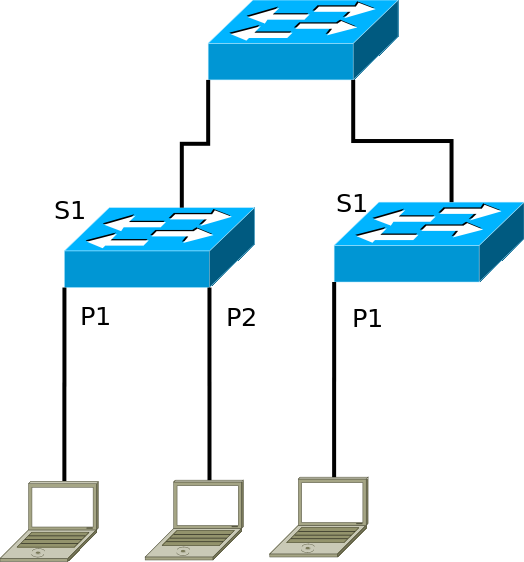
\includegraphics[width=0.4\textwidth]{network_ex2.png}
\caption{Grafik mit Switches, Ports und Host}
\label{fig:network_ex2}
\end{figure}


Für das Auslesen der Switches soll das Netzwerkprotokoll SNMP verwendet werden, da eine Abfrage per Telnet die Switches stark belastet und daher es passieren kann, dass der Betrieb eingeschränkt wird. Hinzu kommt, dass ein Auslesen per Telnet sehr langsam ist und die Ausgabe selbst nicht standardisiert ist und somit sehr viele Einzelfälle behandelt werden müssten.\\\\
Im Hinblick auf die Geschwindigkeit des Auslese-Prozesses wurde vorausgesetzt, dass das Sammeln der Daten mindestens vier Mal am Tag möglich sein muss und sofern möglich sollte eine Auslesezeit unter 60 Minuten angestrebt werden, da es sich hierbei um einen alten Wert handelt, welcher bei früheren Auslesevorgängen erreicht wurde.\\\\
Eine weitere Anforderung die als optional angesehen wird, ist die Möglichkeit die Verbindungen zwischen den Switches und Routern zu erfassen. Das heißt, es soll eine Topologie anhand der Daten erstellt werden können.\\\\
Zu den optionalen Anforderungen gehört die Möglichkeit einer Benutzerzuordnung zu den jeweiligen Hosts. Die Zuordnung soll über das bestehende Active Directory passieren und somit die Möglichkeit bieten den entsprechenden Nutzer bei Problemen direkt anrufen zu können.\\\\
Kombiniert man diese Anforderungen, so bildet sich eine weitere Anwendungsmöglichkeit und zwar kann es in der Praxis vorkommen, dass ein Switch gewechselt und somit abgeschaltet werden muss.
Hierfür kann man nun im Voraus kontrollieren, welche Hosts an diesen angeschlossen sind und welche Nutzer somit im Voraus informiert werden müssen.\\\\
Neben den Anforderungen zu den Anwendungsmöglichkeiten wurden auch Anforderungen an das Programm selbst gestellt.
Zu diesen gehört die Betriebssystemunabhängigkeit.
Das Programm muss sowohl auf Windows-, als auch auf dem Linux-Betriebssystem funktionieren. Sofern Interpretersprachen oder ähnliches verwendet werden, darf keine Versionsabhängigkeit bestehen. Das beudeuten für das Programm, es muss z.B. sowohl unter Java 1.6.0.10 als auch unter 1.6.0.33 funktionieren.\\
Als bestehende Datenbank wurde Oracle vorgegeben, da hierfür bereits Lizenzen existieren und dieses bereits auf den entsprechenden Servern läuft und kein weiteres DBMS installiert und gepflegt werden muss.\\

\section{Anforderungsanalyse}
\label{sec:anfanalyse}

Um die Anforderungen bewerten zu können, muss man sich zunächst mit den Technologien vertraut machen und die technischen Möglichkeiten mit den Anforderungen abgleichen.\\\\
Zunächst einmal muss untersucht werden, ob die im Unternehmen befindlichen Switches auch das SNMP-Protokoll soweit unterstützen, um das Auslesen zu ermöglichen.
Dies wurde überprüft und bei vereinzelten Switches musste die Konfiguration angepasst werden, da hier teilweise SNMP deaktiviert oder nur für spezielle Hosts zugelassen war.\\\\
Im nächsten Schritt galt es zu überprüfen, ob die benötigten Informationen per SNMP überhaupt abfragbar sind. Problematisch hierbei ist vor allem, dass Hersteller zwar eigene MIBs bei SNMP verwenden, über diese lassen sich jedoch nicht die gleichen Informationen abfragen, wie über die proprietären Protokolle der Hersteller.
Bei der Überprüfung der Zuordnung zwischen MAC-Adresse der angeschlossenen Ports wurde festgestellt, dass diese zwar möglich ist, aber eine sehr spezielle Vorgehensweise vorrausetzt.\footnote{vgl. Cisco (2005)}\\\\
Problematisch ist vorallem die genaue Zuordnung der Hosts an den korrekten Switch. So kann es sein, dass die MAC-Adresse eines Hosts sowohl auf einem Access-Switch als auch auf einem Distribution-Switch zu finden ist.
Hierfür muss eine eindeutige Identifizierung stattfinden, welcher Switch welche Hierarchieebene angehört. Diese Informationen müssten manuell gepflegt werden oder anhand einer automatischen Hierarchieerkennung erhalten werden.\\\\
Die Anforderung alle Hosts hinter einem Port zu finden, stellt kein Problem dar, da dies von allen Switches per SNMP unterstützt wird.\\\\
Eine Historie, die es ermöglicht, nur neue Kombinationen aus MAC-Adresse des Hosts und des zugehörigen Ports als neuen Eintrag zu sehen ist, ohne Probleme möglich und kann durch die demensptrechende Erstellung der Datenbank sichergestellt werden.\\\\
Neben den Anforderungen die sich auf die Systemstruktur beziehen, gibt es auch solche, die sich auf den Ausleseprozess konzentrieren.
In diesem Zusammenhang wurde die Auslesegeschwindigkeit und die Last auf den Switches angeführt.
Aussagen über die Auslesegeschwindigkeit können leider im Voraus nicht getroffen werden, jedoch ist anzunehmen, dass die Geschwindigkeit über der des manuellen Auslesens per Telnet liegen muss, da SNMP nicht verbindungsorientiert ist und somit die Endgeräte weniger belastet werden und der Overhead reduziert ist.
Genauere Aussagen über die Geschwindigkeit lassen sich erst durch Benchmarks machen, welche in Kapitel [Kapitel X] durchgeführt werden.\\\\
Um mögliche Verbindungen zwischen den Switches und Routern zu erfassen, muss es möglich sein, auf einem Port einen Switch zu identifizieren, was per SNMP in Verbindung mit STP und CDP möglich ist.\\\\
Eine Zuordnung der einzelnen Nutzer lässt sich über das Active Directiry per LDAP bewerkstelligen, hierfür muss aber ein spezieller Benutzer eingerichtet werden, der vollständige Leserechte für alle Hosts im Netzwerk besitzt.\\\\
Die Betriebssystemunabhängigkeit ist mit einer Vielzahl von Interpreter-Sprachen (Perl, Phyton, ...) oder einer Platform unabhänigen Sprache (Java, C Sharp/Mono) gegeben.\\\\
Da für alle gängigen Sprachen diverse Datenbankanbindungen angeboten werden, gibt es bei der Wahl des DBMS auf Oracle keine Probleme.\\\\
Insgesamt betrachtet gibt es von der technischen Seite zwar gewisse Schwierigkeiten bei der Implementierung, diese verohindern aber nicht eine Umsetzung des Projektes.\\\\
Ein weiterer wichtiger Punkt sind auch die Ressourcen, da für die komplette Implementierung nur 11 Wochen zur Verfügung stehen.
Für eine Implementierung eines Systems mit diesem Umfang und einer ausreichenden Testphase bei nur einem Entwickler ist dies ein zu geringer Zeitraum.
Da vor der Implementierung und den Tests zuerst einmal der Entwurf und gewisse Design Entscheidungen stehen müssen, wird es hier zu Engpässen kommen, welche nur durch Kompromisse im Hinblick auf die Implementierung und den Tests gelöst werden können.\\\\
Da ein Großteil der Zeit für das Auslesen der Daten aufgebracht werden muss, wird die Zeit für die Umsetzung der Weboberfläche deutlich geringer angesetzt, wie die für eine Umfassende Umsetzung notwendig wäre.
Hier muss dann im Laufe des Projektes zwischen einzelnen Funktionen der Weboberfläche abgewägt werden.\\\\
Im Hinblick auf die Kosten entstehen bei der Umsetzung keine weitere Kosten bzw. bei der Wahl eines existierenden Open Source-Systems.
Ziel des Projektes ist das bestehende kommerzielle Produkt zu ersetzen und somit eine monetäre Einsparung, aber auch der Anforderung einer gewissen Modularität gerecht zu werden.\\

\section{Betrachtung bereits existierender Lösungen}
\label{sec:exitloesungen}

Betrachtet man die bereits existierenden Lösungen zum Überwachen von Switches und Hosts, so lassen sich einige Produkte finden, die kommerzieller Natur als auch Open Source sind.
Bei HP Openview handelt es sich um eine kommerziell Lösung von HP, die dazu dient eine komplette Netzwerk und Systemmanagement-Lösung anzubieten. Diese Software-Umgebung besteht nicht nur aus HP eigenen Modulen sondern auch von verschiedenen Fremdherstellern.
Die wichtigste Komponente des HP Openview für die Netzwerküberwachung stellt der sogenannte ‘HP OpenView Network Node Manager’ dar.
Dieser ermöglicht es, neben dem Überblick über die Netzwergeräte und deren Stati zusätzlich detailierte Informationen zu den einzelnen Geräten anzuzeigen.
Diese Daten können bei Bedarf als Histogramme angezeigt werden, z.B. für den aktuellen Daten-Durchsatz an.
Ebenso bietet sich die Möglichkeit einer Art Übersichtskarte die automatisch anhand der vorhandenden Netzwerkgeräte generiert wird. Die notwendigen Informationen hierfür werden per SNMP und CDP ausgelesen. Zusätzlich wird zur Statusüberprüfung auf Funktionen wie ein Ping zurückgegriffen\\\\
Eine weiteres kommerzielles System ist CiscoWorks von Cisco. Dieses bietet untere anderem ein spezielles Usertracking-Modul, welches einem ermöglicht, alle Hosts in einem Netzwerk zu identifizieren, aber auch die dazugehörigen Switches, an die jeweils die Geräte angeschlossen sind anzuzeigen. Diese Informationen können teilweise auch per CDP (Cisco Discovery Protokoll) ausgelesen werden.
Über die per CDP bereitgestellten Daten wird auch ein automatisches sequentielles Auslesen aller Switches im Netzwerk ermöglicht, ohne zuvor diese zu kennen, jedoch müssen die notwendigen Zugangsdaten trotzdem zur Verfügung gestellt werden.\\\\
Das Open Source Programm Nagios dient vor allem zum Überwachen von verschiedenen Geräten im Netzwerk, sowie deren Dienste.\footnote{vgl. Barth, W. (2008), S. 66+96}
Hierbei arbeitet es ebenfalls per SNMP, jedoch ist es aber nicht auf dieses allein angewiesen.
Sofern eingerichtet, kann es auch einfach per TCP oder UDP die Dienste überprüfen.
Es können aber auch Remote Skripts per SSH aufgerufen werden.
Jedoch ist hierbei zu beachten, dass Nagios nur das Überwachen von bekannten und zuvor konfigurierten Hosts und Diensten unterstützt und somit für die gewünschte Anforderung nicht in Frage kommt.\\\\
Ein System , welches die Anforderungen teilweise erfüllt, ist Tirith.
Dieses Programm wird vom Fraunhofer Institut eingesetzt im Kompetenzzentrum Netzwerkmanagement und ist Open Source.\footnote{Siehe: http://www.cc-lan.fraunhofer.de/projekte/tirith/ - Aufruf der Seite: 07.02.2011}
Es unterstützt das Auslesen von diversen Cisco Switches sowie deren jeweiligen Hosts.
Zusätzlich liest Tirith eine Großzahl an Infromationen über die Switches sowie das bestehende VLAN aus.
Funktionen die Tirith nicht bietet, sind ein paralleles Auslesen der Switches und es verfügt auch nicht über eine Historie, wenn ein Port an einem Switch getauscht werden sollte.
\footnote{vgl. Müller, J., (2004), Abbildung 1}

\section{Entscheidung zur eigenen Programmierung}
\label{sec:decisionowncreating}

Vergleicht man alle aufgeführten Systeme, so lässt sich feststellen, dass keine der genannten Lösungen den Anforderungen entspricht.
Zwar bietet Tirith einen Teil der gewünschten Funktionen, jedoch müsste dies erst auf die speziellen Bedürfnisse angepasst werden, die das Unternehmen benötigt.
Aufgrund dieser Tatsache empfiehlt sich eine eigene Implementierung, da diese die Möglichkeit gibt, besonders auf die Anforderungen einzugehen und keine Einarbeitungszeit in eine fremde System-Architektur notwendig macht.
Selbstverständlich sind mit einer eigenen Implementierung gewisse Risiken verbunden, darunter auch der knappe Zeitrahmen.
In der Anforderungsanalyse wurden diese aber bereits abgewegt und eine Machbarkeit des Systems festgestellt.

\chapter{Entwurf und Implementierung}
\label{cha:entw_imp}

\section{Entwurf}
\label{sec:Entwurf}


\subsection{Usecases}
\label{subsec:usecases}

Zu Beginn einer Systementwicklung müssen die Usecases und die beteiligten Akteure identifiziert werden.
Hierfür wird zu Beginn überlegt, welche Personen Zugang zum System haben und welche Aufgaben diese am System erfüllen werden.
Für den Entwurf wird nicht nur die Anforderungsdefinition zu Rate gezogen, sondern der Verfasser bespricht die notwendigen Funktionalitäten, die das Programm später beinhalten soll, mit den Mitarbeitern selbst.
Dadurch kommen meist weitere Punkte auf, die zuvor nicht angesprochen wurden, jedoch wichtig sind für den späteren Entwurf des Systems, sowie die Umsetzung.
In Abbildung \ref{fig:UML_usecases} ist das Usecase-Diagramm für das System zu sehen.

\begin{figure}[H]
\centering
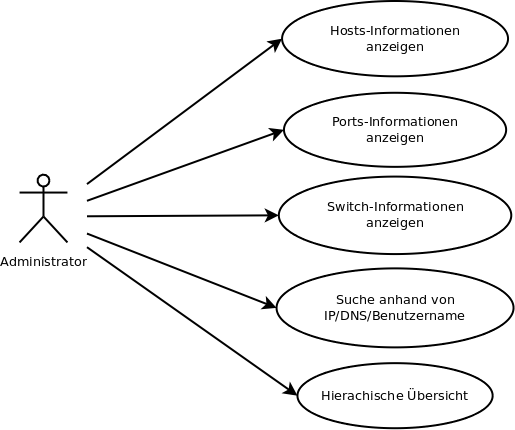
\includegraphics[width=0.8\textwidth]{UML_usecases.png}
\caption{Usecasediagramm}
\label{fig:UML_usecases}
\end{figure}

Zum einen ist festzustellen, dass es nur einen Akteur gibt. Das liegt daran, dass keine Einschränkung vorgesehen ist für die aktiven Nutzer des Systems.
Bei der Implementierung wird jedoch eine mögliche spätere Einführung von verschiedenen Benutzerrechten bedacht und diese Funktionalität als Möglichkeit offen gelassen.
Zur Einfachheit halber wird der Netzwerkdaminstrator im Laufe des Textes als Benutzer beschrieben.
Die erste Sicht, die dem Nutzer zur Verfügung stehen muss, ist eine Übersicht über alle Switches, hier muss neben der Switch IP auch der per SNMP ausgelesene Alias stehen, aber auch die vorhandene IOS-Version und die Seriennummer des Switches.\\\\
In einer weiteren Sicht soll eine Übersicht auf die Ports eines Switches geben werden.
Neben der MAC-Adresse des Ports, sowie des Port Namens (z.B. Fa0/1) sind weitere Informationen sichtbar, unter Anderem der Status (Up/Down), Geschwindigkeit des Ports, Duplexmodus, sofern zugewiesen die VLAN ID, aber auch Informationen, ob es sich hierbei um ein Uplinkport handelt.
Zusätzlich wird eine Sicht benötigt, die Informationen über den angeschlossenen Host anzeigt.
Hierunter fallen Informationen, wie MAC-Adresse, IP, DNS, sowie der zuletzt angemeldete Benutzer an einer Workstation. Zusätzlich sollen aber auch Informationen angezeigt werden, welche in Verbindung mit dem Port in Verbindung stehen. Diese werden im Zuge der Historie zusätzlich beim Host gespeichert.
Sofern es sich um ein CDP-fähiges Gerät handeln sollte, werden diese zusätzliche Informationen ebenfalls angezeigt.
Neben den Sichten zu den Geräten wird es auch eine Übersicht der VLANs geben, welche es erlaubt, eine Verbindung zwischen der VLAN ID und des jeweiligen VLANs herzustellen.
Somit kann nicht nur der Alias sondern auch die entsprechende VTP-Domäne abgelesen werden.\\\\
Der Benutzer soll weiterhin auf jeder dieser Sichten eine Möglichkeit zur Suche eines Hosts/Switches haben, wie auch eine Option zur Sortierung der Einträge.
Neben diesen grundlegenden Funktionen wurde empfohlen, zusätzlich eine Art hierarchische Übersicht zu ermöglichen. Das heißt, der Nutzer kann über die Switchübersicht einen Switch selektieren und erhält dann die Übersicht der dort verfügbaren Ports. Wählt er nun einen Port auf diesem Switch aus, so erhält er alle Hosts die an diesen Port angeschlossen sind.
Sofern es sich dabei um mehrere Hosts handelt, wählt er wiederum einen aus und landet schließlich in der Übersicht über den Host mit den detailierten Informationen.\\\\
Als optionaler Usecase wird das Anzeigen einer Art Dashboard gesehen.
In diesem werden Informationen zusammen gefasst, die nicht direkt erkenntlich über die einzelnene Sichten sind. Beispielsweise könnte man hier Informationen anzeigen lassen, wie z.B. Anzahl freier Ports, Switch mit den meisten freien Ports, Switchs mit der höchsten Auslastung, um nur eine Liste der potentiellen Informationen zu nennen.

\subsection{Klassendiagramme}
\label{subsec:classdiagrams}

Für die Umsetzung des Projektes wurde eine objektorientierte Programmiersprache gewählt, welche es erfordert Klassen zu verwenden.
Diese dienen dazu, Objekte abzuleiten und die jeweiligen Methoden von diesen zu nutzen.
Um das System zu entwerfen wurden 25 Klassen verwendet, da eine möglichst hohe Abstraktion erwünscht war.
Zusätzlich muss auch sichergestellt werden, dass die Beziehungen zwischen den Klassen modular sind, damit ein einfacher Zugriff und eine Austauschbarkeit gegeben ist.
Um ein Einblick in die Struktur des Projektes zu erhalten wird in diesem Kapitel auf die wichtigsten Klassen des Projektes eingegangen.
Die Abbildungen der Klassen befindet sich aus Platzgründen im Anhang.\\\\
Das Ausleseprogramm wird als Objekt der Klasse \textit{SNMPTrack} instanziiert, welche auch den Namen des Auslese-Programms repräsentiert.
Hierbei handelt es sich um die Ausgangsklasse, welche die Steuerung des Programms beinhaltet. Von dieser Klasse aus, wird, wie später in Kapitel \ref{subsec:seqdiagrams} beschrieben, ein Objekt der Klasse \textit{SwitchListe} erzeugt.
Dieses stellt alle Switches inklusive deren Passwörter in einer Liste zur Verfügung.
Das Einlesen dieser Daten erfolgt anhand einer existierenden XML-Datei oder einer bestehenden Datenbank die in der Konfiguration hinterlegt wurde.
Somit wird sichergestellt, dass für das Auslesen im Hauptteil des Programms nur ein Befehl benötigt wird und die Logik separat liegt.\\\\
Neben den Zugangsdaten für die Datenbank werden über die Klasse \textit{SNMPConfig} weitere Informationen zur Verfügung gestellt.
Sie liest anhand der XML-Konfigurationsdatei aus, welche Anzahl von Threads gleichzeitig maximal aktiv sein darf und enthält auch Informationen über das Debug-Level, welches den Detailgrad der Meldungen reguliert.
Durch diese Klasse stehen die Informationen in allen anderen Klassen und Methoden zur Verfügung.\\\\
Die nächste wichtige Klasse ist die \textit{SNMPHandler} , welche alle SNMP Abfragen verwaltet.
Diese Klasse dient dazu, den Abruf eines SNMP Wertes oder sofern notwendig eines ganzen Unterbaums durchzuführen.
Hierfür stellt diese eine Methode bereit, die anhand der gewünschten OID, der IP des SNMP-Agenten, sowie des notwendigen Community-String, die benötigen Informationen  zurückliefert.
Die Rückgabewerte werden in einem speziellen Format zurückgeliefert, um eine spätere Bearbeitung zu vereinfachen. Zum besseren Verständnis dient das nachfolgende Beispiel:\\

<OID>!<Wert>\\

Mit reellen Daten gefüllt, könnte ein Rückgabewert wie folgt sein:\\
\\
1.3.6.1.2.1.1.1!Linux WRT54G 2.4.20 2 Thu Dec 9\\
\\
Durch das Zusammensetzten mit ! kann eine einfachere Verarbeitung stattfinden bzw. der Wert auch manuell besser gelesen werden.
Für das Auslesen eines Switches wird jeweils ein Objekt der Klasse \textit{SwitchWorkerThread} erzeugt. Hierbei handelt es sich jeweils um einen separaten Thread, dem jeweils das \textit{Switch}-Objekt aus der Liste des \textit{SwitchListe} Objekts übergeben wird.
Der Thread ruft anschließend die Methode refresh() der Klasse \textit{Switch} auf.
Diese Methode beginnt daraufhin alle relevanten Informationen eines Switches über die \textit{SNMPHandler} Klasse, wie in Kapitel \ref{subsec:acitvitydiagrams} beschrieben, auszulesen.
Hierzu verwendet die Methode eine programminterne OID-Bibliothek. Diese wird über die Klasse \textit{OIDL} bereitgestellt. Im Detail enthält die Klasse verschiedene Strings, deren Variablenname dem Namen der OIDs im RFC 1213 übereinstimmt.\\\\
Somit kann auf einfache Art und Weise ein übersichtlicher Befehl in den notwendigne String übersetzt werden, wie im folgenden Beispiel:\\
\\
OIDL.vtpVlanName\\
den String:\\
1.3.6.1.4.1.9.9.46.1.3.1.1.4\\
\\
Dies ist vor allem notwendig um eine Übersicht über die verwendeten OID zu behalten bzw. erkennen zu können welcher Wert hinter der jeweiligen OID steckt. Der nachfolgende Quellcode-Abschnitt verdeutlicht die Wichtigkeit der Aliase:\\

\begin{figure}[H]
\centering
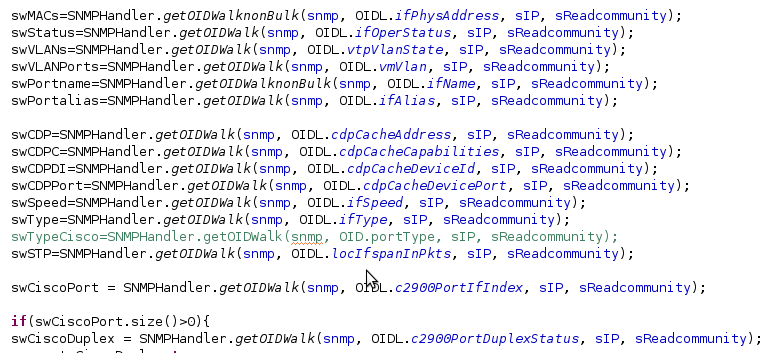
\includegraphics[width=1.0\textwidth]{code_example_OIDL.png}
\caption{Codebeispiel}
\label{fig:classdiagramcode}
\end{figure}

Neben den zuvorgenannten Klassen, gibt auch eine Menge an Klassen, die s ausschließlich als Schnittstelle zu anderen Datenquellen dienen.
Hierzu gehört die Klasse \textit{Nagios}, die es ermöglicht Switches, inklusive Zugangsdaten und deren Gruppenzugehörigkeit, anhand einer existierenden Datenbank mit Daten eines Nagios-Systems auszulesen.\\\\
Eine weitere Schnittstelle stellt die Klasse \textit{LDAP} dar. Diese ermöglicht das Auslesen der Active-Directories der Windows Domäne.
Die Klasse \textit{DNSHelper} ermöglicht es den DNS Namen anhand einer IP zu finden, in dem jeweils der DNS-Server angesprochen wird.\\\\
Für die Kommunikation mit der Datenbank wurde eine spezielle Klasse \textit{DataManagerOracleMulti} erstellt, die es ermöglicht SQL-Befehle die keine Rückgabe erwarten in Stapel auszuführen.
Dies bedeutet, dass die Datenbank nicht jeden Befehl einzeln erhält sondern eine große Anzahl (>100 Stück) auf einmal und somit weniger Overhead für den Verbindungsaufbau entsteht.\\\\
Neben der Vielzahl an Klassen, die einer Vereinfachung des Programmablaufs dienen, gibt es trotzdem Objekte welche auch die Realtät abbilden.
Dazu gehören die Klassen \textit{Switch} (welche bereits beschrieben wurde), \textit{Port}, sowie \textit{Host}.
Diese bieten jeweils Methoden an, welche von sich selbst die passenden SQL-Befehle anhand der enthaltenen Daten generieren. Dies macht es einfacher die Objekte zu serialisieren.
Das heißt, die Objekte im Programm wiederum abzubilden auf eine Textuale-Ebene, um sie in die Datenbank übertragen zu können.\\


\subsection{Sequenzdiagramme}
\label{subsec:seqdiagrams}

Um die Beziehungen der einzelnen Klassen des Programms zu visualisieren, reicht es nicht aus, die Klassendiagramme zu zeichnen, sondern es müssen auch Sequenzdiagramme erstellt werden.
Im Folgenden soll auf die Beziehungen ausgehend von der Hauptklasse des Programms eingegangen werden.
Zu Beginn des Porgramms erzeugt die Klasse SNMPTrack ein Objekt der Klasse SwitchListe.
Bei diesem Objekt wird die Methode getSwitches() aufgerufen.
Diese Funktion liefert dann eine Liste aller Switches, die später anhand einer vorgegebenen Datenquelle ausgelesen werden müssen.
Zum aktuellen Zeitpunkt ist dies eine XML-Datei, in naher Zukunft werden diese Daten anhand des existierenden Nagios Systems ausgelesen. Im Anschluss wird ein Objekt der Klasse SwitchWorkerThread erstellt, um einen separaten Thread zu starten, der unabhängig und nebenläufig arbeiten kann. Dieser Thread nimmt das übergebene Switch Objekt und ruft bei diesem die refresh() Methode auf, welche wiederum für das Einlesen aller Switchinformationen zuständig ist.
Dieser Vorgang ist in Abbildung \ref{fig:sequecediagram1} beschrieben.


\begin{figure}[H]
\centering
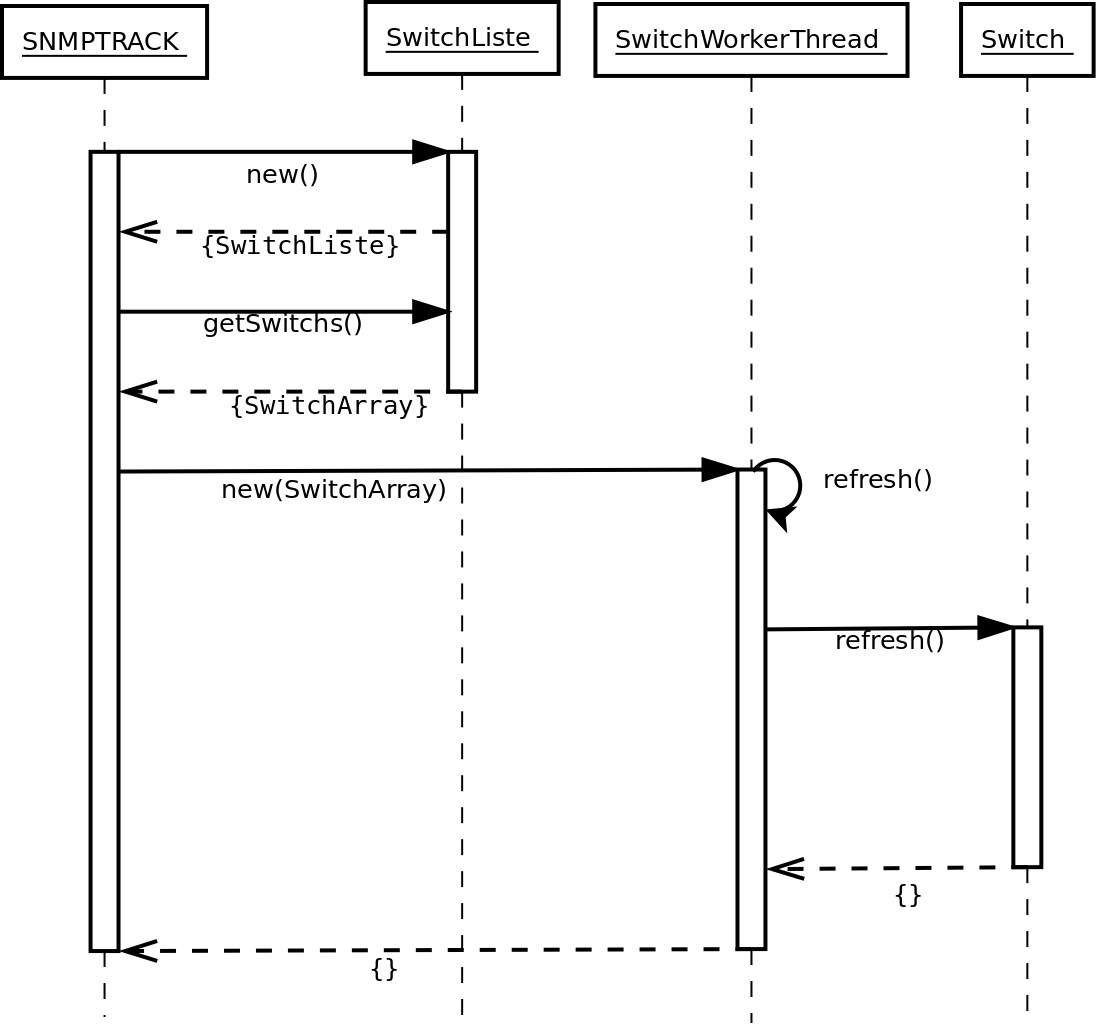
\includegraphics[width=0.7\textwidth]{seq.png}
\caption{Sequenzdiagramm 1}
\label{fig:sequecediagram1}
\end{figure}

Während des refresh() Methoden-Aufrufs des Switch Objektes werden verschiedene andere Objekte erzeugt. Zu Beginn wird die Klasse SNMPHandler verwendet, welche verschiedene Methoden zur SNMP-Kommunikation zur Verfügung stellt. Über diese werden SNMP-GET und SNMP-BULK Befehle abgesetzt. Zusätzlich bietet die Klasse Funktionalitäten, welche SNMP selbst nicht zur Verfügung stellt. Möchte man z.B. den kompletten Unterbaum eines Knoten erhalten und überschreitet die Anzahl der Einträge das Maximum von GETBULK, so können diese nur durch GET und GETNEXT ausgelesen werden. Diese Problematik behandelt die Klasse in einer SNMP-WALK Methode, welche die gleiche Funktionsweise wie ein GETBULK hat, aber es ermöglicht auch größere Listen an Werten abzufragen, die an einem Knoten hängen. Nachdem die jeweiligen SNMP Methoden die Werte zurückgegeben haben, werden diese ausgewertet. Im Anschluss daran, wird ein Objekt der Klasse Port abgeleitet.
Dieses Objekt dient dazu die portspezifischen Informationen zu speichern und im Anschluss den passenden SQL-Befehl zur Speicherung zu generieren. Dies wird durch die Methoden setValues() und saveinDB() realisiert.
Beim Aufruf der saveInDB() Methode kommt es zur Verwendung der Datenbank-Klasse JDBC-Oracle. Diese überträgt den SQL-String an die Datenbank, nachdem die Methode executeSQL() aufgerufen wurde.
Die gleiche Abfolge findet auch mit dem Objekt der Klasse Host statt. Hierbei werden anstatt wie beim Objekt der Klasse Port portspezfische Informationen abgelegt, sondern in diesem Fall die Informationen, welche den jeweiligen Host betreffen, abgespeichert.
Nachdem alle Ports und Hosts abgespeichert wurden, ist die Methode refresh() des Switch-Objektes beendet.\\\\
Jedoch muss bedacht werden, dass während der Verarbeitung der Daten eine Vielzahl von Klassen aufgerufen werden, welche speziell für das Programm geschrieben wurden.
Ein Beispiel stellt die Klasse mit dem Namen Cisco dar, welche Methoden zur Verfügung stellt, die speziell auf SNMP-Daten von Cisco-Geräten anwendbar sind.
Darunter fallen Umformatierungen, die für das Auslesen der Uptime und des Switch Modells notwendig sind.


\begin{figure}[H]
\centering
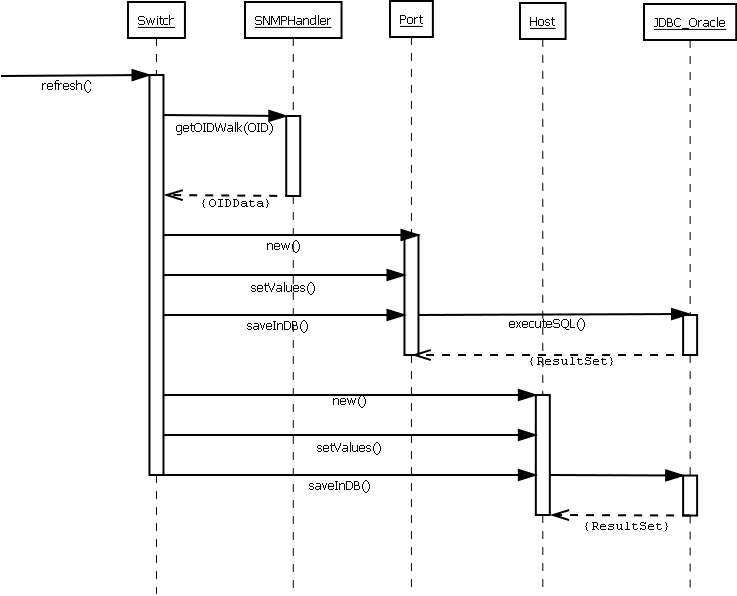
\includegraphics[width=0.9\textwidth]{seq2.png}
\caption{Sequenzdiagramm 2}
\label{fig:sequecediagram2}
\end{figure}

\subsection{Aktivitätsdiagramme}
\label{subsec:acitvitydiagrams}

Zur Darstellung des Programmablaufs eigenen sich vor allem Aktivitäts-Diagramme von der UML.
In Abbildung \ref{fig:activitydiagram1} ist das Diagramm, welches das Hauptprogramm beschreibt, zu sehen..\\

\begin{figure}[H]
\centering
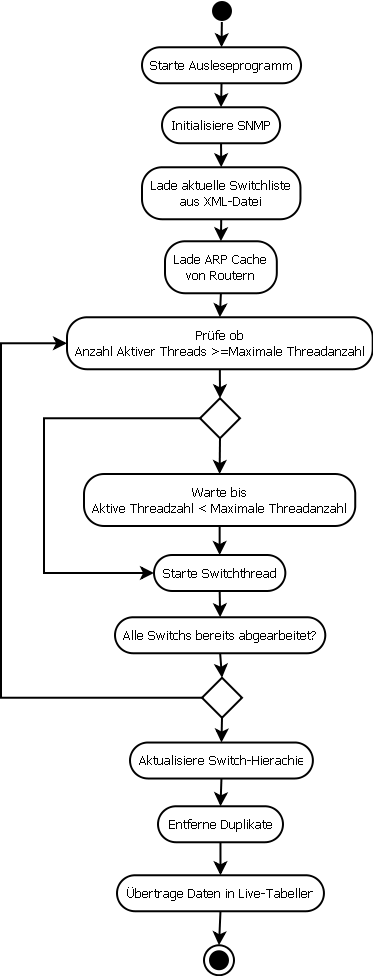
\includegraphics[width=0.45\textwidth]{activity_diagram.png}
\caption{Aktivitätsdiagramm 1}
\label{fig:activitydiagram1}
\end{figure}

Im folgenden Abschnitt, soll dieses näher beschrieben werden.
Anzumerken ist, das es sich bei der Darstellung um eine merkliche Vereinfachung des Programmablaufs handelt, da eine detaillierte Beschreibung den Umfang dieser Arbeit überschreitet. Zusätzlich wurde aus Gründen der Übersichtlichkeit und des verwendeten Programms von der UML-Notation abgewichen. \\\\
Zu Beginn des Programms wird die SNMP-Schnittstelle initialisiert, um das Auslesen der Switches zu ermöglichen. Darauf hin werden die Switches, welche ausgelesen werden sollen, anhand einer existierenden XML-Datei oder einer Datenbank erfasst. Durch diese Datenquelle werden auch die notwendigen Zugangsdaten ausgelesen, die für den Zugriff benötigt werden.
Anschließend wird der ARP-Cache von den Routern eingelesen, der es später ermöglicht, anhand einer MAC-Adresse die passende IP-Adresse zu erhalten.\\\\
Der nächste Abschnitt des Programms steuert die einzelnen Ausleseprogramme, da für jeden Switch ein separater Thread gestartet wird, der unabhängig von den anderen Arbeiten kann. Durch diese Nebenläufigkeit ist ein deutlicher Geschwindigkeitsvorteil bezüglich der kompletten Auslesezeit erwarten.
Jedoch muss ein Kontrollemechanismus existieren, der diese Threads verwaltet. Der Mechanismus überprüft zunächst die Anzahl der aktiven Threads. Liegt diese unter dem definierten Maximalwert, wird ein neuer Thread gestartet. Ist dies nicht der Fall, so wartet dieser, bis die Anzahl der aktiven Threads unter den Maximalwert sinkt und startet danach einen neuen Thread.
Nach jedem Start eines Threads wird überprüft, ob noch weitere Threads gestartet werden müssen und je nachdem entweder wiederholt dieser die Prozedur erneut oder setzt das Hauptprogramm fort.\\\\
Im Anschluss werden werden die Hierarchielevels der Switches anhand der Nagios-Datenbank geupdatet. Dies ist für die nachfolgende Duplikatsentfernung notwendig.
Bei dieser werden Duplikate in der Datenbank untersucht und bei Bedarf gelöscht.
Duplikaten sind die Hosts, die auf mehr als einem Port gesichtet wurden. Hierbei kann es sich um ein Rechner, der an einen neuen Port angeschlossen wurde oder um einen Switch handeln.
Da Switches mehr als ein Interface haben, tauchen diese auch mehrmals in der Liste auf. Der Grund hierfür lieht darin, dass nicht auf allen Switches eine Uplink-Port Erkennung unterstützt wird. Nach dem die Hosts auf den unerkannten Uplink-Ports entfernt wurden, werden alle Daten in die sogenannten ‘Live’-Tabellen übertragen. Diese Übertragung ist notwendig,  da während des Ausleseprozesses die Daten nicht konsistent in der Datenbank vorliegen. Durch dieÜbertragung wird auch sichergestellt, dass während des Ausleseprozesses die Datenbank trotzdem nutzbar vom User ist und dieser keine Ausfallzeit des Systems bemerkt.\\\\

In Abbildung \ref{fig:activitydiagram21} ist der erste Teil des Aktivitätdiagramm des Ausleseprogramms zu sehen.
Die Notation ist wie in Abbildung \ref{fig:activitydiagram1} angepasst.
Der Auslesevorgang lässt sich in drei Teile aufteilen. Zuerst werden die Informationen des Switches, dann die der Ports und letztendlich die der Hosts ausgelesen.
Zuerst wird überprüft, ob der Switch SNMP unterstützt, ansonsten wird das Programm beendet.
Ist dies der Fall werden die Informationen über den Switch ausgelesen und anhandessen der SQL-Befehl erzeugt, der zwischengespeichert wird, um die Vorteile der Datenbank-Transaktion zu nutzen, welche in Kapitel \ref{sec:designent} näher erläutert werden.\\\\
Im nächsten Teil Werden alle Informationen über die Ports ausgelesen.
Dann wird im Anschluss für jeden Port überprüft, ob dieser eine MAC-Adresse hat und kein virtuelles Interface ist, trifft dies nicht zu wird der jeweilige Port verworfen.
Anschließend wird anhand der Informationen von CDP und STP entschieden, ob es sich hierbei um ein Uplink-Port handelt und diese Informationen hinterlegt. Daraufhin wird wiederum der passende SQL-Befehl generiert und zwischengespeichert.

\begin{figure}[H]
\centering
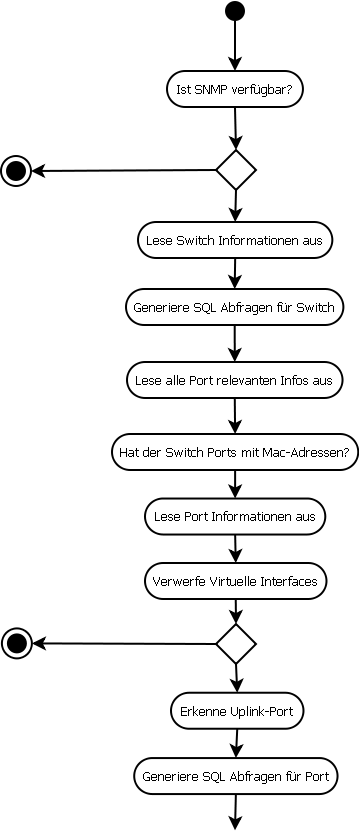
\includegraphics[width=0.5\textwidth]{activity_diagram_switch_thread_01.png}
\caption{Aktivitätsdiagramm 2 - Teil 1}
\label{fig:activitydiagram21}
\end{figure}

Im letzten Teil des Auslesevorgangs werden, wie in Abbildung fig:activitydiagram22 zu erkennen, die Hosts erfasst.
Zu Beginn wird überprüft, ob am jeweiligen Port ein Gerät angeschlossen ist, sollte keins angeschlossen sein wird der Port übersprungen. Ist jedoch ein Gerät angeschlossen, so wird unterschieden ob es sich hierbei um ein Uplink-Port handelt. Ist dies der Fall, so werden die per CDP ausgelesenen Informationen verwendet um den Hosteintrag zu erstellen.
Handelt es sich bei dem Gerät um ein normales Gerät, dass keine CDP Informationen enthält, so wird der Hosteintrag anhand der per SNMP ausgelesenen Informationen erzeugt.
Hierzu wird die MAC-Adresse mit dem zuvor ausgelesenen IP-Adressen des ARP-Cache verknüpft. Anhand dieser IP-Adresse wird wiederum der DNS-Name vom DNS-Server angefordert und sofern es sich um ein Computer des Active Directories handelt, wird zusätzlich der Benutzer ausgelesen.
Auf Grundlage dieser Daten wird wiederum ein SQL-Befehl generiert, der anschließend zwishcengespeichert wird.\\\\
Bevor der Switch-Thread beendet wird, werden die Abfragen aus dem SQL-Puffer an einen speziellen Datenbank Thread übergeben der sich anschließend um das Absetzen der SQL-Befehle kümmert. So kann der Switch Thread bereits beendet werden und im Hauptprogramm das Auslesen des nächsten Switches begonnen werden, auch wenn noch nicht alle Datensätze in der Datenbank sind. Dies dient vor allem der Reduzierung der Wartezeit und somit einer Reduzierung der Auslesezeit.

\begin{figure}[H]
\centering
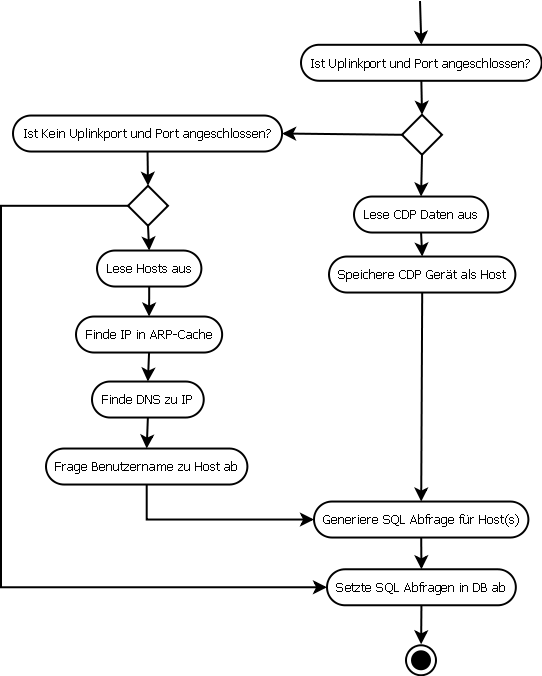
\includegraphics[width=0.7\textwidth]{activity_diagram_switch_thread_02.png}
\caption{Aktivitätsdiagramm 2 - Teil 2}
\label{fig:activitydiagram22}
\end{figure}

\subsection{Enitity Relationship Model}
\label{subsec:erm-diagram}

Aufgrund der vorherigen Analysen ist ein Enitity Relationship Model (ERM) erstellt
worden. Zum Erstellen wurde das Programm Dia verwendet, welches nicht der Chen
Notation folgt, aber eine einfache und schnelle Erstellung einer schemenhaften Abbildung ermöglicht und auch flexibel gegenüber Veränderungen ist.
Der Entwurf der Datenbank als ERM ist in Abbildung \ref{fig:erm} zu sehen.

\begin{figure}[H]
\centering
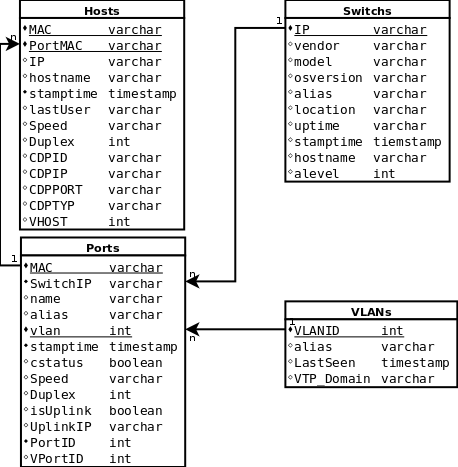
\includegraphics[width=0.7\textwidth]{ERM.png}
\caption{ERM}
\label{fig:erm}
\end{figure}

Um alle Daten verwalten zu können, werden vier verschiedene Tabellen benötigt.
Zunächst wird eine Tabelle zum Speichern der VLAN-Informationen benötigt.
Hierzu existiert die Tabelle VLANs mit dem Primärschlüssel VLANID, welcher für jedes VLAN im Netwerk eindeutig ist und somit auch als Primärschlüssel geeignet ist. Über diesen Schlüssel werden alle VLAN relevanten Informationen abgelegt. Dazu gehören neben dem Namen bzw. Alias des VLANs auch die VTP-Domain und ein Zeitstempel, um unterscheiden zu können, welche VLANs eventuell in der Vergangenheit aktiv waren und in der Gegenwart nicht mehr existieren.\\\\
Die Tabelle Switches dient dazu, alle Switch relevanten Informationen zu speichern. 
Um den Switch eindeutig zu identifizieren reicht die IP Adresse des Switches aus. Über diese werden anschließend Informationen über den Switch gespeichert. Dazu gehören IOS-Version, Modell, Ort, Uptime, aber auch Hostname, sofern vorhanden und die entsprechende Hierarchiestufe, welche anhand des Nagios-Systems ausgelesen wurde.\\\\
In der Port Tabelle werden alle Ports der Switches gespeichert. Die Ports selbst sind eindeutig über ihre jeweilige MAC-Adresse identifizierbar, jedoch soll ein neuer Eintrag angelegt werden, sofern sich die VLAN Einstellung ändert.
Daher dient nicht nur die MAC-Adresse als Primärschlüssel, sondern auch die VLAN ID.
Neben dem Namen des Ports und der MAC-Adresse gibt es auch ein Fremdschlüssel, welcher die IP des angehörigen Switches enthält, um eine eindeutige Zuordnung des Ports an einen Switch zu ermöglichen.
Zusätzlich sind Attribute des Ports bezüglich des Status untergebracht.
So ist zum Beispiel möglich, zu sehen, ob der Port gerade Up oder Down ist, mit welcher Geschwindgkeit auf dem Port kommuniziert wird und welcher Duplex Modus aktiv ist. Auch wird gespeichert, ob es sich bei dem Port um einen Uplinkport handelt.\\\\
In der Host-Tabelle werden alle im Netzwerk befindlichen Hosts gespeichert.
Zur eindeutigen Identifikation der Hosts genügt die MAC-Adresse, jedoch geht aus der Anforderungsdefinition hervor, dass sofern der Host an einen anderen Port angeschlossen wird ein neuer Eintrag angelegt werden muss, daher wurde nicht nur die MAC-Adresse des Hosts, sondern auch die MAC-Adresse des Ports am Switch als Primärschlüssel genommen. Neben den üblichen Informationen wie IP und DNS-Hostname, werden auch Teile des Port Status abgespeichert, da man, sofern der Host an einem anderen Switch angeschlossen wird (z.B. ein Notebook der den Accesspoint wechselt), immernoch wissen möchte, mit welcher Geschwindigkeit dieser PC ursprünglich angeschlossen war. Es reicht aber auch schon das Suchen eines PCs der gerade ausgeschaltet ist.
Um trotzdem herauszufinden, mit welcher Geschwindigkeit dieser angeschlossen war, ist diese Differenzierung notwendig. Zusätzlich dazu werden Informationen abgespeichert, sofern CDP Informationen über den Host bekannt sind. Hier werden dann CDP-Gerätetyp und der CDP-Port gespeichert, dies ist vor allem hilfreich bei Switches, Routern und Firewalls die das CDP Protokoll unterstützen, um eine bessere Einordnung zu erhalten.
Neben diesen Informationen wird im Feld VHOST zusätzlich vermerkt, ob es sich bei diesem Host um einen physikalischen Host oder um einen logischen Host handelt. Das heißt, handelt es sich bei dem Host um einen virtuellen Server wird dieser explizit als Vhost markiert. Erkannt werden alle gängigen virtuellen Hosts. Dazu zählen mit VMWare, Virtualbox, VirtualPC, aber auch mit Parallels (Virtual Desktop, Server, Virtruzzo) oder Xen erzeugte Hosts. Zu beachten ist jedoch, dass z.B. das spezielle VMWare ESXi Server Betriebssystem selbst über eine virtuelle Schnittstelle kommuniziert, also das Host-System selbst und nicht die Gast-VMs.


\section{Design Entscheidungen}
\label{sec:designent}

Für die Umsetzung des Projektes müssen verschiedene Entscheidungen bezüglich der Umsetzung getroffen werden. Einige der Entscheidungen sind entweder durch die Anforderungen spezifiziert oder müssen unter Abwegung der Vor- und Nachteile ausgewählt werden.\\\\
Zuerst muss eine Entscheidung fallen, welche Programmiersprache gewählt wird. Nachdem Abgleich der Anforderungen und der Absprache mit der Fachabteilung, standen Perl und Java zur Auswahl. Da einer der Anforderungen auch die Geschwindigkeit betrifft, wurde zuerst eine Test Applikation in beiden Sprachen geschrieben.
Dieses hat jeweils einen Switch mit wenig Netzwerk-Traffic mit einer Vielzahl von SNMP Abfragen beschäftigt, um Benchmakrwerte zu erhalten.\\\\
Im Benchmark-Programm wird die Zeit gemessen, wie lange es dauert um 1000 Abfragen durchzuführen.
Der in Millisekunden gemessene Wert wird in die nachfolgende Formel eingesetzt:\\

Anzahl der Requests*1000/Benötigte Zeit in ms= Abfragen pro Sekunde\\

Daraus resultiert die jeweilige Anzahl der Abfragen pro Sekunde, welche es ermöglicht einen Vergleich durchzuführen.\\

In der nachfolgenden Grafik sind die beide Programmiersprachen aufgezeichnet:\\

\begin{figure}[H]
\centering
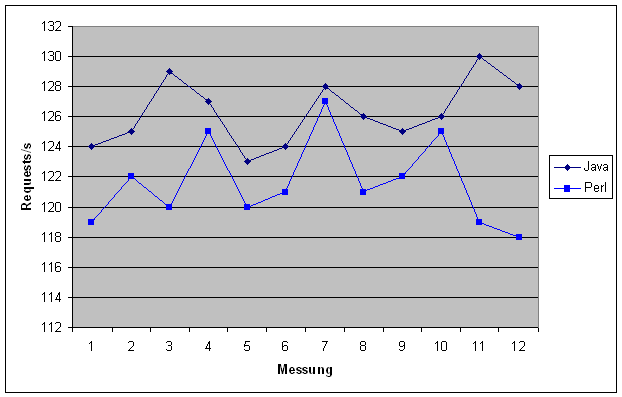
\includegraphics[width=0.8\textwidth]{bench_j_p.PNG}
\caption{Benchmark - Vergleich zwischen Perl und Java}
\label{fig:benchperljava}
\end{figure}

Wie in der Abbildung zu erkennen, liegt Java ein Bruchteil vor Perl.
Der geringe Unterschied zwischen den beiden Programmiersprachen lässt sich dadurch erklären, dass die Implementierung der SNMP-Abfragen minimal anders sind, der bei beiden fast gleich hohe Wert lässt darauf schließen, dass der Flaschenhals des Benchmarks der Switch selbst ist. Dies konnte dadurch validiert werden, wenn beide Benchmarks  gleichzeitig gestartet wurden und dann eine Halbierung beider Benchmark Werte erfolgte.\\\\
Da es somit kein Unterschied macht, welche der beiden Sprachen zum Einsatz kommt, wird die Entscheidung anhand der Möglichkeiten beider Sprachen und deren Modularität gefällt und somit fällt die Wahl auf Java.\\\\
Da unter anderem eine Vielzahl an Switches abgefragt werden muss, empfiehlt es sich, eine Parallelisierung anzustreben, da jeder Switch nur eine begrenzte Geschwindigkeit aufweist.
Hierfür eignet sich die Verwendung von Threads, um den Teil der Abfragen zu parallelisieren, der unabhängig voneinander ablaufen kann.
Um den Nutzen einer Parallelisierung zu validieren, wurde wiederum ein Benchmark durchgeführt. Bei diesem Benchmark wurde die Anzahl der Threads variiert und jeweils die Zeit gemessen.\\

\begin{figure}[H]
\centering
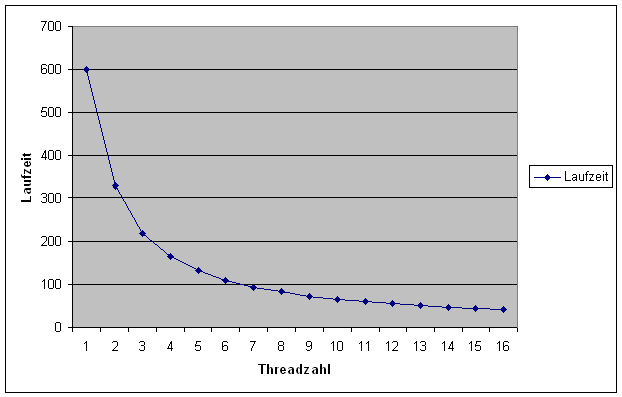
\includegraphics[width=0.8\textwidth]{bench_threads.PNG}
\caption{Benchmark - Parallelisierung}
\label{fig:benchparallel}
\end{figure}

Wie in der Abbildung \ref{fig:benchparallel} zu erkennen ist, lässt sich feststellen, dass durch die Parallelisierung ein bedeutender Geschwindigkeitszuwachs zu messen ist.
Für die Abfragen pro Switch wurden jeweils 2000 Abfragen angenommen, das ein geschätzer Maximalwert pro Switch später darstellen sollte.\\\\
Bei der Durchführung des Benchmarks wurde ist ein Problem  aufgetreten und zwar kam es zu Fehlern bei Thread-Zahlen über 20. Hierbei reicht der UDP-Puffer für die SNMP-Abfragen nicht mehr aus und somit kann der Empfang aller SNMP-Pakete nicht mehr sicher gestellt werden.
Daher empfiehlt es sich bei der Implementierung einen niedrigeren Wert zu wählen und auf Nummer sicher zu gehen.\\\\
Bei der Version 2 des SNMP-Protokolls gibt es einen speziellen Abfrage Modus “BULKGET”. Bei diesem musste auch überprüft werden, in welchem Umfang dieser dem normalen GET ein Geschwindigkeitsvorteil bringt. Hierfür wurden der erste Benchmark angepasst und die Liste der Ports von einem Switch abgefragt, ein Mal alle Ports sequentiell und ein Mal per BULK-Befehl.\\\\
Die Ergebnisse des Benchmarks lassen sich im nachfolgenden Bild erkennen.\\

\begin{figure}[H]
\centering
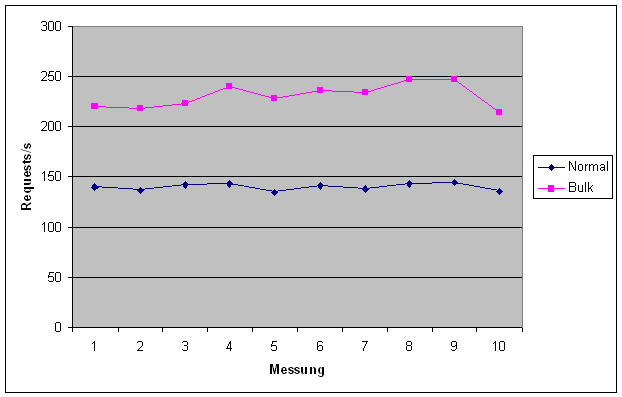
\includegraphics[width=0.8\textwidth]{bench_bulk.PNG}
\caption{Benchmark - SNMP Bulk}
\label{fig:benchsnmpbulk}
\end{figure}

Es lässt sich feststellen, dass der BULK Modus einen bis zu dreifachen Geschwindigkeitsvorteil bringt. Jedoch muss beachtet werden, dass im Falle einer größeren Anzahl von Antworten (ab 50) diese nicht vom BULK Modus zurückgegeben werden, daher ist der Einsatz nur partiell sinnvoll.\\\\
Hierbei muss bei der Implementierung dann genaustens beachtet werden, wann welche Methode eingesetzt werden kann.\\\\
Eine weitere Sache, die überprüft werden muss, ist die Abwegung, ob es sinnvoller ist die SQL-Befehle, welche neue Datensätze hinzufügen, zuerst zu sammeln und mit einem Commit abzusetzen oder aber jeden einzelnen Datensatz separat abzusetzen.
Hierfür wurde ein weiterer Benchmark durchgeführt, um eine Entscheidung in dieser Hinsicht treffen zu können.\\

\begin{figure}[H]
\centering
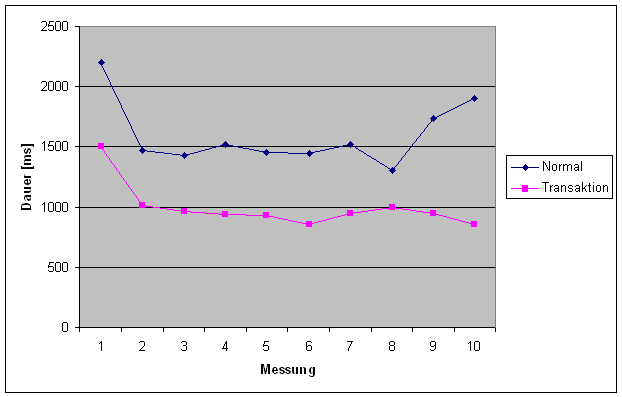
\includegraphics[width=0.8\textwidth]{bench_oracle.PNG}
\caption{Benchmark - Oracle Transaktionen}
\label{fig:benchoracletransactions}
\end{figure}

In Abbildung \ref{fig:benchoracletransactions} ist zu erkennen, dass es von Vorteil ist, die Commits zuerst zu sammeln und dann abzusetzen.
Während des Benchmarks wurde jedoch erkannt, dass durch eine Vielzahl von vorgehaltenen Abfragen, die durch die Parallelisierung entstehen, die Anzahl der gleichzeitig offenen Tabelleneinträgen sich stark erhöht und somit das Limit der Datenbank überschreiten wird.
Zwar wurde anschließend das Limit der maximal offenen Einträge erhöht, jedoch kam es selbst dann zu Überschreitungen.
Daher wurde der Algorithmus so angepasst, dass er immer in Paketen zu je 100 Befehlen arbeitet.
Durch diese Maßnahme ist es trotzdem möglich, einen Geschwindigkeitsvorteil zu erhalten, bei gleichzeitiger Einhaltung der Limits.

\section{Auswahl der Hilfsmittel}
\label{sec:hilfsmittelwahl}

Für die Umsetzung des Projektes sind verschiedene Hilfmittel notwendig.
Zum einen wird eine Entwicklungsumgebung benötigt.
Da die Wahl der Programmiersprache auf Java gefallen ist und kommerzielle Lösungen nicht zur Auswahl stehen, fiel die Wahl auf Eclipse, da es neben NetBeans zu den wenigen Open Source IDEs gehört, welche eine Vielzahl von Erweiterungsmöglichkeiten bietet und interaktive Funktionen wie Code-Vervollständigung oder Code-Vorlagen, aber auch standardmäßige Funktionen wie Syntaxhervorhebung unterstützt.\\\\
Zur Softwareversionverwaltung wurde Subversion verwendet.
Die Auswahl wurde auf ein Open-Source System gelegt und zusätzlich auf ein zentrales System, um ein großes Maß an Interpolität zu erreichen.
Die Wahl fiel speziell auf Subversion, da es im Gegenzug zu CVS das Versionsschema nicht auf einzelene Dateien sondern auf das ganze Projekt bezieht.
Das hat den Vorteil, dass das Hinzufügen einer neuen Funktion nicht in der Hauptklasse Version 50 und in der Methodenklasse Version 70 gespeichert wird, sondern in einer gemeinsamen Version.
Somit ist es für dne Entwickler möglich den Zusammenhang zwischen den einzelnen Dateien direkt zu erkennen, da die neue Funktion z.B. in der Revision 60 in beiden Dateien erkennbar ist.\\

\section{Schnittstellen}
\label{sec:schnitt}

Um ein Projekt mit vielen Einlese- und Exportfunktionalitäten erstellen zu können, werden viele Schnittstellen benötigt.
Zum Einen wird bei diesem Projekt eine Schnittstelle für die SNMP-Abfragen benötigt, zum Anderen wird eine Anbindung an das Active Directory angestrebt. Zusätzlich müssen aber auch alle Datenbankzugriffe sowohl vom Einleseprogramm, als auch von der Website bewerkstelligt werden.\\\\
Im Folgenden wird auf die jeweiligen Schnittstellen eingegangen, wie diese sequentiell im Ablauf des Ausleseprogramms verwendet werden. Diese lassen sich wiefolgt zusammenfassen:
\begin{itemize}
\item Einlesen aller benötigten Konfigurationsdaten
\item Auslesen per SNMP
\item Rekursive DNS Abfragen
\item Auslesen per LDAP
\item Datenbankverbindung Java
\item Datenbankverbindung Webserver\\
\end{itemize}

Die erste Schnittstelle ist beim Start des Programmes zum Auslesen der Daten angesiedelt. Hierbei muss der Benutzer dem Programm eine Großzahl von Informationen übergeben.
Es existiert eine spezielle XML-Datei in der die Switches, welche ausgelesen werden müssen, die Router, welche den ARP-Cache enthalten, sowie die notwendigen Zugangsdaten für die Datenbanken, enthalten sind. \\\\
Das Programm selbst bietet dem Nutzer keine Möglichkeit Übergabe-Parameter zu definieren, damit ein möglichst einfacher Ablauf ermöglicht und zusätzliche Fehleingaben des Benutzers vermieden werden.\\\\
Die nächste Schnittstelle ist die Kommunikation mit den Switches per SNMP. Um nicht die komplette SNMP-Kommnunikation selbst per UDP implementieren zu müssen, empfiehlt es sich hierbei, eine bereits vorhandene API zu nutzen.
Speziell für Java gibt es hierfür unter anderem folgende Möglichkeiten:
\begin{itemize}
\item SNMP4J
\item jSNMP
\item WebNMS SNMP
\item iReasoning SNMP API
\item netsnmpj\\
\end{itemize}

Schließt man nun alle kommerziellen Lösungen aus, so bleiben lediglich SNMP4J und netsnmpj übrig.
Da mehrere SNMP-Abfragen später gleichzeitig durchgeführt werden müssen, ist die Wahl auf SNMP4J gefallen, da dieses threadsicher ist und auch ein größeren Funktionsumfang als netsnmpk bei der Implementierung mit sich bringt.\\\\
Um anhand der ermittelten IP-Adressen die dementsprechende DNS-Namen zu erhalten, ist es notwendig, ein Reverse-DNS-Lookup zu machen.
Hierfür muss das sogenannte JNDI verwendet werden, welches einem erlaubt, selbstdefinierte DNS-Abfragen zu erstellen.
Um beispielsweise den DNS-Namen der IP 192.168.0.1 herausfinden zu können, muss dieser aber erst in ein spezielles Format gebracht werden. Hierzu wird die IP Adresse umgekehrt zu 1.0.168.192 und der Zusatz “.in-addr.arpa” angehängt. Daraus folgt dann:\\

1.0.168.192.in-addr.arpa\\

Diese Adresse wird inklusive dem Modus “PTR”, welche für einen Reverse-DNS-Lookup steht, an den DNS Service Provider übermittelt und das Resultat wiederum zurückgegeben.\\

Für das Auslesen des zugehörigen Benutzers muss das Active Directory befragt werden.
Hierzu gibt es eine Mehrzahl von Möglichkeiten, die jedoch dadurch eingeschränkt werden, dass diese nur unter Windows lauffähig sind. Daher muss auf Ansätze zurückgegriffen werden, bei denen es möglich ist plattformunabhängig zu agieren. Hierzu muss man die Architektur vom Active Directory von Windows genauer untersuchen.\\\\
Generell lässt sich das Active Directory in folgende Komponenten unterteilen:
\begin{itemize}
\item LDAP-Verzeichnis
\item Kerberos-Protokoll
\item Common Internet File System
\item Domain Name System (DNS)\\
\end{itemize}

Hiervon ist vor allem das LDAP-Verzeichnis bedeutend, welches es ermöglicht den Benutzer des jeweiligen Computers herauszufinden.
Da LDAP per RFC genaustens spezifiziert ist (aktuell im RFC 4511) und Microsoft diesen Standard ebenfalls nutzt kann mit einer LDAP-API auf das Verzeichnis zugegriffen werden.
Hierfür bietet Java mit seinen enthaltenen Bibliotheken ebenfalls eine Schnittstelle ähnlich der DNS-Abfragen an. Über diese können die Attribute eines Objektes im Verzeichnis abgefragt und gesetzt werden. In diesem Verzeichnis befinden sich auch die einzelnen Computer als Objekte. Diese wiederum haben diverse Attribute, welche unter anderem auch den aktiven Nutzer enthalten.\\\\
Für die Verbindung des Java-Programms zur Oracle und MySQL-Datenbank gibt es verschiedene Möglichkeiten. Hierzu zählen die verschiedenen Arten von Treibern, die eine Datenbankverbindung ermöglichen. Zu allererst ist die ODBC-Schnittstelle zu nennen, welche es ermöglicht, unabhängig von der eingesetzten Datenbank, die Anbindung an das Programm immer auf die gleiche Art realisieren zu können.
Da diese Unabhängigkeit dadurch erreicht wird, dass die SQL-Befehle erst in die datenbankspezifischen umgewandelt werden müssen und somit ein Overhead entsteht, ist diese Lösung meist langsamer als eine native Lösung. Daher ist es von Vorteil spezielle vom Hersteller angebotene JDBC-Treiber einzusetzen, welche anstelle des JDBC-ODBC Brücken-Treibers den zusätzlichen Overhead meiden und direkt mit dem DBMS kommunizieren.\\\\
Bei der Verbindung mit dem Webserver kann wiederum ein ODBC-Treiber einsetzt werden oder speziell für die Programmiersprache PHP geschriebene Bibliotheken, die es erlauben, ähnlich wie bei Java direkt mit dem DBMS zu kommunizieren um unnötigen Overhead zu vermeiden.

\section{Zeitplan}
\label{sec:timetable}

Für die Umsetzung eines Softwareprojektes ist nicht nur ein Entwurf notwendig, sondern auch die Planung über den zeitlichen Ablauf. Der Faktor Zeit spielt eine wichtige Rolle, da er die beiden Variablen Qualität und Kosten begrenzt. Da bei diesem Projekt keine externen Kosten anfallen werden, kann dieser Punkt des magischen Dreiecks außenvor gelassen werden.
Aufgrund der sehr knappen Zeit war es vor allem wichtig, einen zuvor definierten Plan zu haben, welcher die genauen Schritte spezifiziert. Um einen Überblick über den Umfang des Projektes zu bekommen, lohnt sich wiederum ein Blick auf die Usecases in Kapitel X, sowie die Anforderungsdefinition in Kapitel Y. Diese bilden eine gute und wichtige Basis, um einen Projektstrukturplan zu erstellen, welcher im Projektmanagement eine wichtige Rolle spielt. Aufgrund dieses Planes ist es möglich, die einzelnen Arbeitspakete zu definieren. Eine Zuordnung der Arbeitspakete zu einer Person muss nicht erfolgen, da die Software nur von einer Person entwickelt und umgesetzt wird. Nachdem die Arbeitspakete definiert wurden, mussten diesen jeweils eine Dauer zugewiesen und die jeweiligen Abhängigkeiten angegeben werden.
Bei den Zeitangaben wurden Näherungswerte von bereits umgesetzten Projekten verwendet.
Normalerweise kann eine Ressource (in diesem Fall ein Mitarbeiter) nur immer einem Arbeitspaket aktiv zugewiesen werden, alle anderen Arbeitspakete können immer nur einzeln und nacheinander abgearbeitet werden, nie aber parallel. Aus diesem Grund wurde auch auf eine ausgiebige Planung der Resourcen verzichtet. Viel wichtiger war hingegen die Terminplanung, welche aufgrund der Angaben (Dauer und Abhängigkeiten) anhand der Arbeitspakete erstellt werden kann.
Im nachfolgenden sieht man in Abbildung \ref{fig:zeitnetz1} den Terminplan für das Projekt.

\begin{figure}[H]
\centering
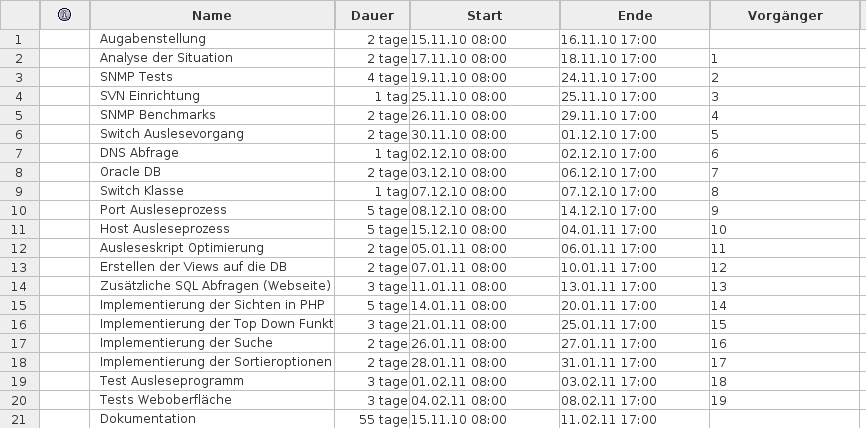
\includegraphics[width=1.0\textwidth]{netzplan1.png}
\caption{Zeitplan - Arbeitspakete}
\label{fig:zeitnetz1}
\end{figure}

Anhand des Terminplans kann wiederum ein Gantt-Diagramm erzeugt werden, welches einen grafischen Überblick über alle Arbeitspakete, sowie deren zeitliche Einordnung, ermöglicht. Das passende Gantt-Diagramm zum Projekt ist in Abbildung \ref{fig:zeitnetz2} zu sehen

\begin{figure}[H]
\centering
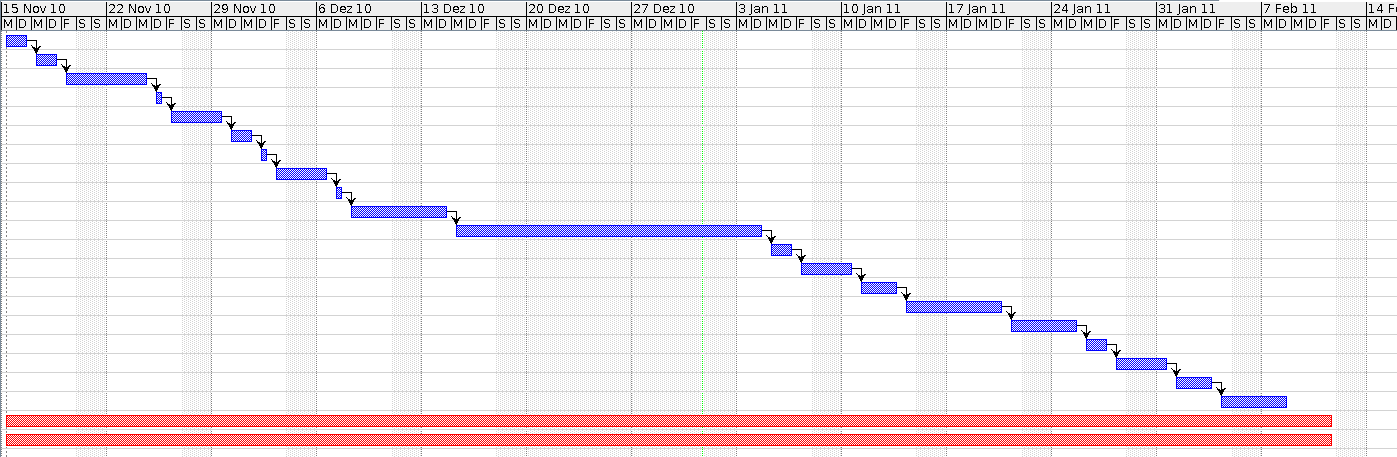
\includegraphics[width=1.0\textwidth]{netzplan2.png}
\caption{Zeitplan - Ganttdiagramm}
\label{fig:zeitnetz2}
\end{figure}

In diesem ist erkennbar, dass das Projekt einen konstanten sequentiellen Ablauf hat.
Zwar hätte die Möglichkeit bestanden, ein paar einzelne Arbeitspakete parallel auszuführen, jedoch in Verbindung mit dem bereits angesprochenen Problem, dass nur eine Person an der Umsetzung arbeitet und diese ein Arbeitspaket nachdem anderen abarbeitet, keine zeitliche Möglichkeit für eine Parallelisierung gegeben ist.
Zu beachten ist auch der rot gefärbte Balken am unteren Ende des Diagramms, welcher als kritischer Pfad angedeutet ist. Hierbei handelt es sich um die Dokumentation. Diese wird zwar als kritischer Pfad angezeigt, aber da die Umsetzung des Projektes sequentiell voranschreitet und immer ein Teil der Dokumentation bearbeitet wird, ist diesem keine weitere Betrachtung zu schenken. Die Zeiten der einzelnen Arbeitspakete sind flexibler anzusehen als diese im Detail definiert wurden, jedoch gibt es hierbei die Einschränkung, dass diese in Summe nicht den Endtermin überschreiten dürfen.

\section{Realisierung}
\label{sec:implementation}

Nachdem sowohl die Umsetzung als auch der zeitliche Ablauf im Detail geplant wurden, konnte mit der Implementierung und somit mit der Realisierung des Projektes begonnen werden.
Zuerst wurde, wie im Zeitplan definiert, das Ausleseprogramm umgesetzt und im Anschluss die dazugehörige Webseite.
Realisiert wurde das System auf einem virtuellen VMWare Server mit dem Betriebssystem OpenSuse (Linux). Als Webserver diente Apache 2 in Verbindung mit PHP 5.3.2. Die PHP Version wurde speziell mit einer Oracle Datenbank Anbindung kompiliert.
Auf diesem Server lief zusätzlich neben dem Webserver ein Oracle Datenbankserver in der Enterprise Edition in Version 11g R2.
Das Ausleseprogramm selbst läuft betriebssystemunabhängig und mit einer beliebigen Java Version ab dem Jahre 2006. Zusätzlich ist es unerheblich, ob das Programm mit der original Sun Java VM ausgeführt wird oder mit dem quelloffenen OpenJDK, welches bevorzugt in Linux-Distributionen eingesetzt wird.
Beim Start des Ausleseprogramms wird zunächst überprüft, ob die Datei Switch.xml existiert und bei Bedarf diese ausgelesen, welche wiederum die Switches inklusive deren Read-Community enthält. Ist die Datei nicht existent, werden die auszulesenden Switches anhand der Nagiosdatenbank ausgelesen. Die Daten für die Nagiosdatenbank, sowie für die Oracle Datenbank, in der später die Informationen abgelegt werden, befinden sich in der config.xml.
Diese enthält neben der maximalen Threadanzahl auch die Einstellung für den SNMP Intervall, der in Kapitel \ref{sec:designent} angesprochen wurde.
Dieser Intervall dient zur Reduzierung der Last auf den Switches während des Auslesevorgangs.
In der Konfigurationsdatei ist ebenfalls ein Parameter zu finden, welcher es ermöglicht, ein Debuglevel zu setzen.
Je nach Höhe dieses Levels werden nicht nur Fehler, sondern auch Warnungen, Hinweise oder auch Meldungen ausgegeben.
Die Levels lassen sich wie folgt einordnen:\\
\begin{itemize}
\item Level 0: Anzeige von Fehlern
\item Level 1: Zusätzliche Anzeige von Warnungen
\item Level 2: Zusätzliche Anzeige von Hinweisen und Warnungen
\item Level 3: Alle Meldungen\\
\end{itemize}

Zusätzlich werden alle Meldungen, die per Programm ausgegeben werden, auch in der Log-Datei gespeichert.
Diese Meldungen sind abhängig vom Loglevel.
\\
\begin{figure}[H]
\centering
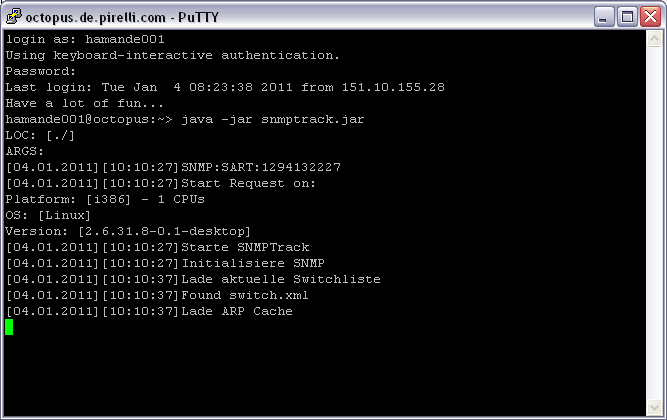
\includegraphics[width=0.8\textwidth]{snmptrack_start.png}
\caption{Programm - Ausleseprogramm}
\label{fig:snmptrack_start}
\end{figure}
In Abbildung \ref{fig:snmptrack_start} ist der Start des Programms zu sehen. In diesem ist auch zu erkennen, dass keinerlei Parameter übergeben wurden. Dies wurde in der Art realisiert, um Bedienfehler zu vermeiden und die Ausführung per Skripte zu erleichtern.
Zusätzlich werden fehlerhafte Einträge innerhalb der XML-Dateien einfach ignoriert.\\\\
Die Weboberfläche des Systems wurde per PHP realisiert.
Bei dieser kommen Cascading Style Sheets und Java Script zum Einsatz.
Um die Zeit für die Implementierung zu veringern, wurde auf die freie CMS Tints zurückgegriffen und diese dementsprechend angepasst.\footnote{Tints, http://sourceforge.net/projects/tints-system/ - Aufruf der Seite: 07.02.2011}
\\
\begin{figure}[H]
\centering
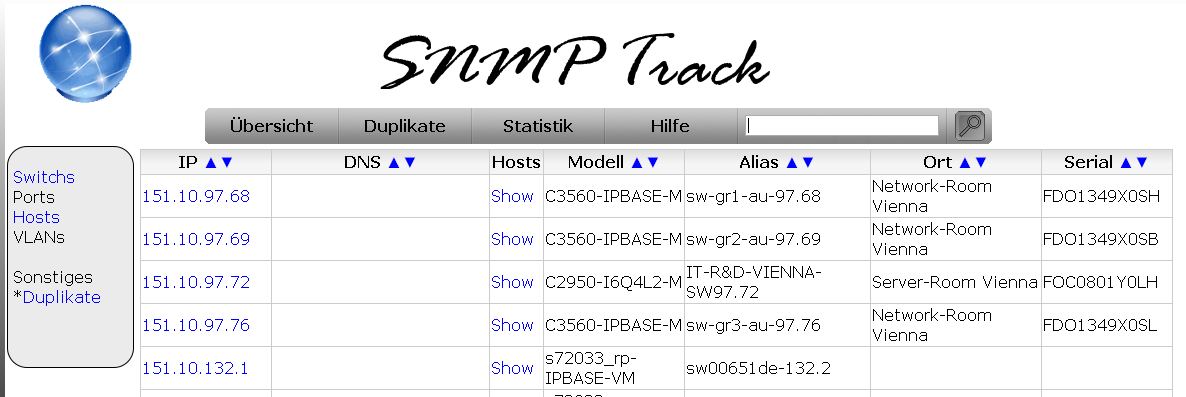
\includegraphics[width=1.0\textwidth]{snmptrack_overview.png}
\caption{Programm - Weboberfläche}
\label{fig:snmptrack_overview}
\end{figure}
Die Oberfläche in einem frühen Stadium der Entwicklung ist in Abbildung \ref{fig:snmptrack_overview} zu sehen.
Neben dem Grundgerüst für die Darstellung der Tabellen müssen spezielle SQL-Abfragen erstellt werden, da später eine Sortierung aller Spalten möglich sein muss.
Diese Sortierung wird durch die Übergabe der GET-Parameter realisiert. Klickt der Benutzer auf eine Spalte wie in Abbildung \ref{fig:snmptrack_overview} zu sehen, so wird der GET-Parameter ‘sort’ in folgendem Format übergeben:\\
\\
sort=model\_A\\
\\
Hierbei stellt ‘model’ 1:1 den Spaltennamen der zu sortierenden Spalte dar und 'A' gibt die Sortierrichtung an. In diesem Fall steht A für das englische Wort ‘ascending’, d.h. aufsteigend. Für eine absteigende Sortierung wird ‘D’ angegeben für ‘descending’.
Zusätzlich gibt es in der Weboberfläche die Möglichkeit, sich Duplikate in der Datenbank anzeigen zu lassen.
Hierbei handelt es sich um Rechner, die auf zwei unterschiedlichen Ports im Netzwerk auf der selben Switch-Ebene gefunden wurden.
Bei diesen Einträgen handelt es sich um 90\% der Fälle um Hosts, welche den Port im Netzwerk gewechselt haben.
In der Praxis bedeutet dass, das ein Notebook, der per WLAN verbunden ist, die Access Points oder ein Computer die Abteilung gewechselt.

\section{Probleme bei der Implementierung}
\label{sec:probimp}

Während der Implementierung traten verschiedene Probleme auf, welche berücksichtigt werden mussten, um abschließend trotzdem alle gewünschten Anforderungen alle umsetzen zu können.
Die Probleme lassen sich vor allem zu den folgenden Punkten einordnen:\\
\begin{itemize}
\item Zuordnung Host --> Switchport
\item Verwendete VLANs
\item Uplinkport-Identifizierung
\item Differenzierung der Switchlevels
\item SNMP-Abfragen und CPU-last auf den Switches
\end{itemize}

Als erstes Problem ist die genaue Zuordnung zwischen Host und Switchport zu nennen.
Hierbei hat sich während der Implementierungsphase gezeigt, dass die Daten, welche per SNMP auslesbar sind, nicht denen gleichen, die lokal auf den Switches per Telnet über das Cisco System zu erhalten sind. So kann das Cisco System einem direkt anzeigen, welche MAC-Adressen sich hinter welchem Port verbirgt. Über SNMP sind diese Informationen jedoch nicht direkt erhaltbar, hier müssen erst verschiedene abrufbare “Tabellen” verknüpft werden. Als erstes müssen die verwendeten VLANs des Switches abgefragt werden (die Problematik der VLAN Abfrage wird im anschließenden Absatz erläutert).
Danach muss eine Liste der MAC-Adressen auf den virtuellen Ports pro VLAN abgefragt werden. Diese einzelnen Listen müssen miteinander kombiniert werden und alle Duplikate entfernt werden. Im Anschluss muss diese Liste mit einer weiteren Liste, welche die Zuordnung zwischen Port und virtuellen Port enthält, verknüpft werden. Aufgrund dieser Liste kann dann eine Verbindung zwischen MAC-Adresse des Ports und der MAC-Adresse des Hosts hergestellt werden. Durch diese Komplexität steigt die Anzahl der Abfragen deutlich, um die gleichen Informationen zu erhalten.\\\\
Eine weitere Problematik stellte sich beim Auslesen der verwendeten VLANs. Es besteht die Möglichkeit per SNMP eine Liste abzufragen, welche ermöglicht, das verwendete VLAN für den jeweiligen Port zu erhalten. Ports die mehrere VLAN Zuordnungen haben, werden nicht angezeigt und sind Trunk-Ports, welche eigentlich Uplink-Ports sind bzw. an solche angeschlossen sind. In diesem Zusammenhang stellt sich die Problematik, dass es passieren kann, dass zwar ein Port für eine spezielles VLAN festgelegt wurde, jedoch sich dahinter noch ein VOIP-Telefon befindet, dass über ein “nicht sichtbares” VLAN kommuniziert, welches über die Liste im SNMP nicht erkennbar ist. Um trotzdem die MAC-Adresse des VOIP-Telefons zu erhalten, müssen alle im Netzwerk bekannten VLANs an einem Switch abgefragt werden, was wiederum die Anzahl der Abfragen erhöht, aber auch eine Problematik mit sich bringt. In diesem Zusammenhang gibt es spezielle Cisco spezifische VLANs, die sich im Bereich 1002-1005 befinden, welche ausgeschlossen werden müssen, da eine Abfrage der MAC-Adressen dieser VLANs zu einem Timeout führt und unnötig den Ausleseprozess verzögert.\\\\
Die Identifizierung der Uplink-Ports an den Switches stellte ebenfalls ein Problem dar. Hier gibt es keine einfache anwendbare Regel. Zuerst wurde angenommen, dass jeder Trunk Port ein Uplink Port ist. Diese Annahme war jedoch falsch, da in dem vorher aufgeführten Beispiel sich dahinter auch ein durchgeschleifter Computer an einem VOIP-Telefon befinden kann. Daher scheidet das Attribut “Trunk-Port” als solches zur Identifizierung aus. Das nächste Attribut, welches ausgewählt wurde, ist ein spezielles Cisco spezifisches Protokoll mit dem Namen CDP. Es dient dazu Cisco Geräte an einem Port zu identifizieren. Um einen Uplink Port zu identifizieren, wurde dann angenommen, dass sofern das Protokoll CDP vorhanden ist, es sich hierbei um einen Switch handelt. Hier stellt sich jedoch die Problematik, dass es auch Geräte gibt, die auf CDP antowrten, welche weder Switches noch Router sind. Ein Beispiel sind VOIP-Telefone, die es auch von Cisco gibt. Daher wurde zusätzlich die Typerkennung des CDP Gerätes abgefragt, welche Auskunft über diverse Eigenschaften des Gerätes gibt.
Über diese kann überprüft werden, ob es sich hierbei um einen Switch handelt. Leider hat sich in der Praxis gezeigt, dass dieses nicht vollständig ausreicht, da nicht alle Switches sämtliche Abfragen unterstützen, somit musste nach einer zusätzlichen Identifikationsmöglichkeit gesucht werden.
Hier ist der Verfasser auf die Möglichkeit gestoßen, dass Spanning Tree Protokoll per SNMP abzufragen. Dieses ermöglicht die Kommunikation zwischen den einzelnen Switches, um unter anderem Pfadkosten der einzelnen Verbindungen auszutauschen. Nun wurde per SNMP die Anzahl der ausgehenden STP-Pakete auf dem jeweiligen Port ausgelesen und dieses als weiteres Kriterium eingeführt, über welches eine Identifikation des Portes ermöglicht wird und zusammen in Kombination mit CDP eine sehr verlässliche Identifikation zur Verfügung stellt.\\\\
Ein weiteres Problem hat die Einordnung der Hierarchieebenen der Router dargestellt. Um Duplikate reduzieren zu können, ist es notwendig, zu wissen, ob die MAC-Adresse eines Hosts auf einem Uplink/Downlink Port eines Switches erkannt wurde oder an seinem normalen Port. Hierzu muss man wissen, ob der Switch ein Access-Switch ist oder ein Switch einer höheren Ebene.\\
Die Hosts im Netzwerk sind, mit einer geringen Anzahl von Ausnahmen, alle an Access-Switche angeschlossen.
Zusätzlich gibt es Endgräte, die auch an die Distribution-Switches angeschlossen sein können, z.B. die Server im Rechenzentrum. 
Um diese Problematik lösen zu können, wurden die Hierarchieebenen jeweils numerischen äquivalenten Zahlen zugeordnet.
Hierzu wurden die Core Switches mit der Zahl 0, die Distribution Switches mit der Zahl 1 und die Access Switches mit der Zahl 2 definiert.
Da die Information der Ebene des Switches nicht direkt von diesen selbst auslesbar ist, gibt es effektiv nur zwei Möglichkeiten.
Zum Einen kann man die komplette Hierarchie anhand der Uplink Ports mit einem Programm logisch abbilden.
Dazu müsste man einen Hauptknoten auswählen und anhanddessen eine Einordnung der Switches erfolgen lassen, was jedoch äußerst komplett ist und den Zeitlichen Rahmen de Projektes sprengt.
Zum Anderen besteht die Möglichkeit diese Informationen von einer extern Quelle einzulesen, wovon auch gebraucht gmeacht wurde.
In diesem Zusammenhang wird das bereits existierende Nagios System im Unternehmen verwendet. Zu diesem wird mittels JDBC zu einer MySQL Datenbank eine Verbindung aufgebaut, über diese dann im Anschluss die Gruppeninformationen der zu kontrollierenden Hosts, in diesem Fall der Switches, ausgelesen werden. Die Switches sind in verschiedene Host-Gruppen einsortiert, unter anderem auch in die benötigten Access, Distribution und Core Hierarchien. Über diese Gruppen werden die jeweiligen Hosts bzw. Switches erfasst und deren Hierarchielevel in der Datenbank eingetragen.\\\\
Neben den hauptsächlich logischen Probleme zur Identifikation stellte sich unter anderem noch ein weiteres Problem bei der Abfrage der Informationen per SNMP heraus.\\
Wie bereits in vorherigen Kapitel angedeutet, werden die auszulesenden Switches bei SNMP-Abfragen besonders belastet, weshalb eine Erhöhung der Anzahl von Abfragen stehts kritisch in den Ausführungen bewertet wurde.
In der Beschreibung zur Zuordnung zwischen MAC-Adresse des Hosts und der MAC-Adresse des Switches von Cisco, wird diese Problematik nicht angesprochen, jedoch gibt es von Cisco weitere Informationen zu der Problematik, speziell bei einem Artikel zum Auslesen der CPU-Last per SNMP. In diesem wird angeführt, dass die Abfrage des Wertes selbst zu einer Verfälschung des Wertes führt. Zudem wird empfohlen nicht mehr als 1 Abfrage pro Sekunde per SNMP auf einen Switch zu machen, da geringere Intervalle bereits zu Beeinträchtigungen führen.
Vergleicht man dies mit den Benchmarks aus Kapitel X, so lässt sich feststellen, dass diese Grenze beim Ausleseprozess um ein hundertfaches überschritten wird. Es muss auch bedacht werden, dass die Switches nicht für solche Operationen konzipiert wurden, sondern vielmehr für ihre eigentliche Aufgabe, insofern ist das Ziel die Last auf den Switches möglichst gering zu halten, um den Netzwerk-Betrieb in keinster Weise zu beeinflussen. Aufgrund eines logischen Fehlers im Programmablauf kam es während diverser Tests dazu, dass einer der Core-Switches übermäßig ausgelastet war und dies dazu geführt hat, dass das Überwachungsystem der Switches anschließend Warnungen versendet hat. Solche Fälle dürfen im Betrieb nicht passieren, da die Ursache für die hohe Last der Switches nicht erkennbar ist und neben der Störung des Betriebes auch zusätzlich für Verwirrung sorgt. Daher ist es wichtig, die Anzahl der Abfragen per SNMP auf ein Minimum zu halten und im späteren Verlauf der Implementierung weiter zu optimieren, sofern sich Möglichkeiten ergeben.

\section{Tests}
\label{sec:tests}

Im Zuge der Implementierung müssen diverse Tests durchgeführt werden. Hierzu kommen neben dem obligatorischen Test der kompletten Implementierung, Tests welche Teile des Programm testen oder aber auch Tests die als Basis für Entscheidungen dienen.
Im Nachfolgenden soll darauf eingegangen werden, welche Tests explizit durchgeführt werden müssen und welche Ergebnisse diese Tests hatten bzw. welche Konsequenz daraus gezogen wurden. Hierbei wird chronologisch vorgegangen, um die Tests in der Reihenfolge aufzuführen, in der sie für die Realisierung benötigt wurden.\\\\
Zu Beginn des Projektes standen mehrere Tests an, welche diverse APIs überprüft haben. Diese dienten dazu, sicherzustellen, dass eine Kommunikation über die benötigten Schnittstellen erfolgreich ist. Darunter sind Tests gefallen, wie die Überprüfung von SNMP4J, aber auch die des Programmcodes zum Reverse-DNS-Lookup, Abfrage des Active Directory oder die  Überprüfung der Datenbank-Anbindung. Das Ergebnis der Überprüfungen hat dazu geführt, dass eventuell eine andere API verwendet werden musste, sofern ein Test nicht erfolgreich war oder spezielle Einstellungen gemacht werden mussten.\\\\
Nachdem die APIs und Grundfunktionalitäten überprüft wurden, kam es zu den nächsten Tests. Diese dienten zur Entscheidungsfindung über die Nutzung von speziellen Algorithmen oder Design-Entscheidungen, wie sie in Kapitel \ref{sec:designent} angeführt wurden.
Die erste Entscheidung, die getroffen werden musste, war die Wahl der Programmiersprache. Hier zu wurde ein Benchmark des SNMP Aufrufs durchgeführt und die Anzahl der maximalen  Abfragen pro Sekunde miteinander verglichen. Das Ergebnis war, dass die Programmiersprache als solche keinen Einfluss auf die Auslesegeschwindgikeit hat, da der Flaschenhals der Switch selbst darstellt. Der nächste Test der durchgeführt wurde, war die Überprüfung, ob eine Parallelisierung den gewünschten, zuvor prognostizierten Geschwindigkeitsvorteil erbringt. Das Ergebnis dieses Tests war, dass die gleichzeitige Ausführung des Programmcode antiproportional im Bezug auf Anzahl der verwendeten Threads und Laufzeit wirkt. Jedoch traten bei einer bestimmten Anzahl zunehmend Fehler aufgrund des Pufferüberlaufs auf. Dies führte dazu, dass die Anzahl der gleichzeitig aktiven Threads auf ein Maximum begrenzt wurde. Neben der Parallelisierung wurden auch die Auslesemethoden von SNMP selbst überprüft. So wurde getestet, ob eine Geschwindigkeitsverbesserung erreicht wird, wenn der SNMP-Bulk Modus, welcher in Version 2c spezifiziert wurde, verwendet wird.
Das Ergbnis dieses Tests war eine dreifache\footnote{vgl. Kapitel X} Leistungssteigerung, aber auch die Erkenntnis, dass per SNMP-Bulk nur eine begrenzte Anzahl von Tabelleneinträgen abfragbar ist. Diese Information war wiederum wichtig für die Implementierung des Ausleseskripts und hat zur Vermeidung von potentiellen Fehlern im Betrieb geführt. Ebenfalls überprüft wurde die Möglichkeit, mehrere Datensätze gesammelt an die Datenbank zu übertragen.
Ziel war es, zu überprüfen, ob dies den Overhead der einzelnen Verbindungen reduziert und generell für einen Geschwindigkeitszuwachs sorgt. Aufgrund des Benchmark wurde festgestellt, dass dies der Fall ist, jedoch Probleme auftreten, da die Anzahl der gleichzeitig geöffneten Tabelleneinträge stark erhöht wird. Im Fall der einzelnen Abarbeitung und bei einer maximalen Anzahl aktiv arbeitender Switchthreads von N beläuft sich die maximale offene Tabelleneintragszahl auf N.
\\ Bei einer gesammelten Übertragung beträgt die Anzahl der offenen Tabelleneinträge:\\
N*M\\
Wobei N wiederum die Anzahl der maximal aktiven Threads darstellt und M die maximale Anzahl der SQL-Befehle die vom Switch abgesetzt werden müssen. Eine Näherungszahl für M ist:\\
\\
1+52+52*H\\
\\
Wobei hier H die Anzahl der Hosts hinter einem Port ist. Diese liegt in der Praxis durchschnittlich zwischen 1 und 2. Nimmt man hier den Wert 2 an, so ergibt sich für M der Wert:\\
\\
1+52+52*2=157\\
\\
Dieser wiederum eingesetzt in die ursprüngliche Formel ergibt:\\
\\
N*157\\
\\
Für N kann der Wert angenommen werden, der auf Grundlage der Benchmarks in Kapitel \ref{sec:designent} empfohlen wurde.
Das heißt, es wird für N der Wert 10 angesetzt und führt somit zu:
\\
10*157=1570\\
\\
Vergleicht man dies mit dem Wert der gleichzeitig offenen Tabelleneinträge bei einzelner Ausführung von 10, ist ein merklicher Unterschied zu erkennen. Vergleicht man nun die erhaltene Zahl mit dem Standard Wert von 50,\footnote{vgl. Oracle® Database Reference, http://download.oracle.com/docs/cd/B19306\_01/server.102/b14237/initparams138.htm - Aufruf der Seite: 07.02.2011} so lässt sich feststellen, dass der Wert einer gesammelten Durchführung den Standard-Wert um ein vielfaches überschreitet.
Oracle selbst empfiehlt den Wert zu erhöhen und liefert teilweise \footnote{vgl. Oracle Wiki, http://wiki.oracle.com/page/OPEN\_CURSORS - Aufruf der Seite: 07.02.2011} die Oracle Datenbank mit dem Wert 300 aus. Eine Erhöhung des Wertes bringt keinerlei Performencenachteile mit sich, jedoch dient die Begrenzung dazu, um Applikationen, welche die Tabelleneinträge nicht korrekt schließen, daran zu hindern, ein Großteil der Tabellen zu blockieren. Daher wurde der Wert auf 2000 erhöht, um auch die Spitzen im Ausleseprozess abzufangen.\\\\
Neben diesen Tests, welche zu Design Entscheidungen dienten, wurden während der Implementierung durchgängig Tests durchgeführt, die den Funktionsumfang sicherstellen bzw. Funktionen an Ort und Stelle zu überprüfen.\\\\
Der abschließende Test, welcher alle Funktionen des Programms überprüfen soll, wird anhand der Usecases bzw. der Anforderungen abgeleitet. Von diesen wiederum kommt man auch auf die technischen Einzelheiten, wie z.B. das Ausleseprogramm.
Es müssen folgende Programmteile getestet werden:\\
\\
Webapplikation:\\
-Hostinformationen anzeigen\\
-Portinformationen anzeigen\\
-Switchinformationen anzeigen\\
-VLANinformationen anzeigen\\
-Suche anhand von IP/DNS/Benutzername\\
-Hierarchie Übersicht\\
\\
Ausleseprogramm:\\
-Auslesen der SNMP-Informationen\\
-Zuordnung zwischen Host und Port \\
-Zuordnung zwischen MAC und IP\\
-Auflösung von IP zu DNS\\
-Abfrage des Benutzers\\
-Entfernung von Duplikaten\\
\\
Nachdem diese jeweils auf Funktionalität und Korrektheit überprüft wurden, kann das Programm für die Nutzung übergeben werden.\\
\\
Ergebnis der finalen Tests\\
\\
Bei den finalen Tests wurde das komplette zusammengesetzte System als Black-Box-Test getestet.
Dabei wurden alle Usecases durchgeführt und überprüft, ob das erwartete Ergebnis mit dem Erhaltenen übereinstimmt.
Es wurde währendessen festgestellt, dass es passieren kann, dass zwei DNS-Hostnamen einer IP zugewiesen sind. Zuerst wurde vermutet, dass es sich hierbei um ein programminterner Fehler handelt und ein Puffer verwendet wurde, der eventuell nicht geleert wurde. Nach der Durchsicht des Codes konnte jedoch kein Fehler entdeckt werden. Im Anschluss wurden mit Betriebssystemmitteln (nslookup) die DNS-Auflösung überprüft. Hierbei wurde festgestellt, dass das Problem beim DNS-Server selbst liegt. Dieser behält über einen festen Zeitraum die Zuordnung von DNS zu IP.
Jedoch prüft dieser im Gegensatz zum DHCP-Server nicht, ob eine IP bereits vergeben wurde oder doppelt in der Namensauflösung vorliegt. Durch diesen Umstand kann es passieren, dass Hosts die keinen DNS-Namen am Name-Server gemeldet haben einen alten Eintrag übernehmen.


\section{Weitere Anwendungsfelder / Datamining}
\label{sec:otherthoughts}

Neben den Anforderungen die von der Abteilung für das neue System angebracht wurden, gibt es weitere Anwendungsmöglichkeiten. Neben dem Anzeigen der jeweiligen Sichten (VLAN, Switch, Ports, Hosts) und der Suche in diesen ergeben sich weitere Nutzungsmöglichkeiten. Eine bereits erwähnte Möglichkeit ist die sogenannte Top-Down Sicht, welche es ermöglicht die Elemente hierarchisch zu durchsuchen. Ein Klick auf einen Switch öffnet somit die Liste mit allen dessen enthaltenen Ports. Diese sind wiederum auswählbar und führen zu den Hosts, welche an dem jeweiligen Port angeschlossen sind.
Da es sich hierbei um mehre Hosts handeln kann, da eventuell ein WLAN-Access-Point an einen Port angeschlossen ist, muss eventuell einer der Hosts explizit noch einmal ausgewählt werden, um dessen Detailinformationen zu erhalten.
Die Möglichkeit, die sich zusätzlich bietet, sieht es vor, das Modell in die umgekehrte Richtung zu erweitern, sodass auch ein Ablauf der Hierarchie von unten nach oben ermöglicht wird.
So soll der Benutzer über den Host, zu dessen zugehörigen Port und von diesem wiederum zum Switch gelangen.\\\\
Eine weitere Anwendungsmöglichkeit stellt das Anzeigen von statistischen Daten dar.
So könnte berechnet werden, wie viele Switch-Ports aktiv belegt sind oder welche Switches am meisten freie Ports haben oder die wenigsten. Solche oder ähnliche Abfragen könnte man dazu verwenden, wenn neue Hosts im System an Switches angeschlossen werden müssen.\\\\
Zusätzlich bietet sich auch die Möglichkeit potentiell nicht erwünschte Hardware zu erkennen.
Dies ist durch den Abgleich diverser Listen möglich.\\\\
Eine weitere Anwendungsmöglichkeit ergibt sich, wenn die Hosts in Verbindung mit den Ports gespeichert und deren Verknüpfung inklusive des Zeitstempels genutzt werden.
So ist es anhand von diesen Daten machbar, eine Historie zu erstellen, die zeigt, an welchen Switches bzw. deren Ports der Host angeschlossen war. Diese Historie ist chronologisch sortierbar und gibt den “Pfad” des Hosts wieder. Im Beispiel könnte dies ein Notebook sein, welcher an verschiedenen Accesspoints angeschlossen war.
Somit ist nicht nur dessen aktuelle Position erkennbar, sondern auch die vorherig genutzen Ports.
Sofern man alle Switches auf einen Geländeplan grafisch darstellen würde, könnte man farblich den Weg des Notebooks darstellen.
Neben der grafischen Darstellung der Switches auf dem Werksgelände bietet sich durch die, anhand von CDP ausgelesenen, Informationen die Möglichkeit, die Hierarchien zwischen den Switches grafisch dazustellen. D.h. durch die jeweils gespeicherten Uplink IPs auf den Ports kann somit eine Verbindung zu dem jeweiligen Nachbar-Switch hergestellt werden.
Nimmt man nun die Core Switches als Hauptknoten, so kann man einen grafischen Baum bilden, welcher in den Blättern, in diesem Fall den Access Switches, endet.
Theoretisch gesehen könnte man aus den Blättern einen weiteren Knoten machen und den Baum bei den Hosts enden lassen, jedoch leidet in der Praxis vor allem die Übersicht an einer solchen Darstellungsweise. Es wird daher abgeraten diese zu verwenden.

\section{Wirtschaftliche Betrachtung}
\label{sec:economicloverview}

Untersucht man das Projekt hinsichtlich seiner Wirtschaftlichkeit, so muss zunächst die Ausgangsituation betrachtet werden. In dieser existiert die bereits bestehende Lösung CiscoWorks, welche in einer veralteten Version vorliegt. Für diese wurde bereits ein Angebot eingeholt, welches sich auf ungefähr 8000€ bewegt. Sofern hier kein Update durchgeführt wird, können alle neueren Switches nicht unterstützt werden.
Ein weiterer Aspekt ist, dass nur ein Bruchteil der Funktionen, die von CiscoWorks angeboten werden, auch tatsächlich genutzt werden.\\\\
Im Vergleich dazu hat eine selbst entwickelte Lösung keinerlei Lizenzkosten und kann auch neuere Switches unterstützen. Betrachtet man beide Möglichkeiten von der monetären Seite, so lässt sich eine Einsparung von 8000€ erreichen. Jedoch muss bedacht werden, dass eine selbstentwickelte Lösung hingegen mit Arbeitszeit  verbunden ist.  Diese müssen als Kosten angerechnet werden. Jedoch handelt es sich bei diesem Projekt um ein Sonderfall, da die Aufgabenstellung während der Praxisphase des Studenten mit der Bachelorarbeit einhergeht, somit fällt keine zusätzliche Mehrarbeit an, da die betreffende Person in jedem Fall mit dem Projekt beschäftigt sein muss.
Trotzdem ist es sinnvoll zu kalkulieren, in welcher Höhe Kosten bei der eigenständigen Entwicklung entstehen.
Da für eine detailierte Berechnung die Personalkosten eingeplant werden müssen, ist es notwendig zuerst erst ein Stundensatz zu definieren.
Um einen Vergleich erstellen zu können, ist es ratsam die Kosten zu berechnen, wenn das System von einer externe Person und wenn es von einer internen Person erstellt wird.
Vergleicht man die Zahlen für einen Software-Entwickler im externen Umfeld, so lässt sich ein Durchschnittswert von 65€/Stunde festlegen.\footnote{vgl. GULP-Stundesatz Kalkulator, http://www.gulp.de/cgi-gulp/trendneu.exe/MONEYFORMDLL?txtPosition=IT+Allgemein+\&txtFachSchwer=Java+Oracle\&lstvAndOr=und\&resultsample=10 - Abgerufen - 07.02.2011}
Neben den Kosten spielt natürlich der Faktor Zeit ebenfalls eine wichtige Rolle. Für die Umsetzung des Projektes wurde in Kapitel \ref{sec:timetable} eine Annahme getroffen über die Zeit, die benötigt wird, das Projekt umzusetzen. Jedoch muss bei dieser Schätzung bedacht werden, dass hierbei, neben einer Einarbeitungszeit, gleichzeitig eine Bachelorarbeit geschrieben wird und die Erfahrung des Entwicklers nicht auf dem selben Level eines externen Spezialisten ist. Grob geschätzt ist also die Annahme von 50 Werktagen auf ca. die Hälfte reduzierbar. Bei einer Annahme von 30 Tagen (zu je 8 Stunden pro Tag) ergibt sich eine Stundenzahl von 240 für das Projekt.
Verrechnet man diese Stundenzahl mit dem Stundenlohn, so erhält man 15.600€. Dieser Wert liegt deutlich über dem Wert einer neuen Lizenz. Daher ist von einer Umsetzung des Projektes von einem externen Entwickler abzuraten. Für die Umsetzung durch einen internen Entwickler liegen leider keine genauen Zahlenwerte vor, daher wird ein Beispielhafter Wert angenommen, wie er in jedem Unternehmen gültig sein könnte. Für einen Mitarbeiter, der mit allen Kosten (inkl. betrieblicher Anteil der Versicherungen) 5000€ pro Monat Kosten verursacht, lässt sich bei einer durchschnittlichen Zahl von 20 Werktagen pro Monat und einer 40 Stunden Woche, ein Stundenlohn wie folgt berechnen:\\
\\
\(\frac{5000\text{EUR}}{20*8h}=31,25\frac{\text{EUR}}{h}\) 
\\
\\
Berechnet man nun die Kosten für das Projekt für einen internen Mitarbeiter, so lässt sich feststellen, dass die Kosten deutlich gesunken sind:\\
\\
\(31,25\frac{\text{EUR}}{h}=7500\text{EUR}\)
\\
\\
Bei anderen Kosten für interne Mitarbeiter schwankt dieser Wert natürlich. Generell lässt sich jedoch feststellen, dass der Wert, welcher die Kosten für einen Mitarbeiter beschreibt nicht über einen Wert X liegen darf, der sich wie folgt bestimmen lässt:\\
\\
\(\frac{X\text{EUR}}{20*8h}*250=8000\text{EUR}\)\\
\(X=5120\)\\
\\
Somit lässt sich feststellen, dass ab einem Kostenpunkt von ca. 5120€ für einen Mitarbeiter pro Monat dieser die Kosten eines Updates der Cisco Software übersteigt.
Jeder Wert unter diesem Grenzwert kann als unproblematisch angesehen werden.\\\\
In diesem Zusammenhang muss auch betrachtet werden, wie oft ein Update einer solchen Software ansteht.
Generell gibt es bei CiscoWorks verschiedene Versionen.
Sofern es sich um ein Major-Release handelt (1.0 -> 2.0, 2.0->3.0), muss eine neue Lizenz gekauft werden.
Um nun eine Schätzung machen zu können, welche Kosten auf die PD zukommen, wenn fortlaufend Updates für CiscoWorks gekauft werden müssen, ist die Versionsgeschichte von CiscoWorks zu Rate zu ziehen.\footnote{Vgl. diverse Cisco Artikel auf cisco.com}
Diese sieht wie folgt aus:
\\
CiscoWorks 2000 -> 1999\\
CiscoWorks LMS 1.0 -> April 2000\\
CiscoWorks LMS 2.0 -> März 2001 \\
CiscoWorks LMS 3.0 -> Juni 2007\\
CiscoWorks LMS 4.0 -> September 2010\\
\\
Diese Daten ergeben einen Durschnittswert von einer Version in 2,5 Jahren.
Setzt man diesen auf drei Jahre, ist dies dann auch ein realistischer Wert, wenn die beiden letzten Versionen im Bezug gesehen werden. Somit kann man von einem Kostenpunkt von fortlaufend von \(\frac{8000}{3}=2667\text{EUR}\) pro Jahr ausgehen. Mit diesen Werten lässt sich eine grobe Schätzung für die kommenden Jahre bewerkstelligen.
Um ebenfalls der Inflation gerecht zu werden wird eine Inflation von 2\% angenommen, basierend auf der Inflation von 3,06\% der letzten 20 Jahre und der aktuellen Situation.\footnote{vgl. Statistisches Bundesamt (2011)}
%https://www-genesis.destatis.de/genesis/online;jsessionid=EAB152D1233569D94D5BBAD6DD0E8733.tomcat_GO_1_1?operation=previous&levelindex=3&levelid=1297088550526&step=3
Kosten die bei der Wahl der Updates für die nächsten fünf Jahre entstehen:\footnote{Einheiten werden aus Gründen der Übersichtlikeit nachfolgend nur am Endergebnis angefügt}\\
\\
\(2667*(1,02)^{1-1}+2667*(1,02)^{2-1}+2667*(1,02)^{3-1}+2667*(1,02)^{4-1}+2667*(1,02)^{5-1}=13879,18\text{EUR}\)\\
\\
Würde man sich für die Selbsterstellung der Software entscheiden muss man zum Einen die Entwicklungskosten von 240 Stunden und zum Anderen zusätzlich für jeden neuen nicht unterstützen Router eine Anpassungszeit von maximal sechs Stunden berechnen.
Da im Netzwerk nur eine geringe Anzahl von unterschiedlichen Switches im Betrieb ist, ist die Anzahl der Anpassungen pro Jahr im Durchschnitt maximal auf zwei zu sehen.
Die Inflation wird ebenfalls auf den Lohn angerechnet. Für die Kosten auf 5 Jahre gesehen ergibt sich somit:\\
\\
\(31,25*240+2*6*31,25*(1,02)^{1-1}+2*6*31,25*(1,02)^{2-1}+2*6*31,25*(1,02)^{3-1}+2*6*31,25*(1,02)^{4-1}+2*6*31,25*(1,02)^{5-1}=9451,52\text{EUR}\)
\\
\\
Diese Zahl ist zwar höher als die Kosten für eine neue CiscoWorks Version, aber es besteht auch die Möglichkeit fremdartige Switches zu unterstützen.
Beachtet man nun die realen Kosten, so kann man feststellen, dass für die initale Entwicklung keine Kosten entstanden sind, so lässt sich die Rechnung wie folgt aktualisieren:\\
\\
\(2*6*31,25*(1,02)^{1-1}+2*6*31,25*(1,02)^{2-1}+2*6*31,25*(1,02)^{3-1}+2*6*31,25*(1,02)^{4-1}+2*6*31,25*(1,02)^{5-1}=1951,52\text{EUR}\)
\\
\\
Wie sich erkennen lässt, stellt dies nur ein Bruchteil der Kosten eines Updates wieder.
Somit ist die Entscheidung für die Entwicklung eines eigenen wirtschaftlich Systems sinnvoll.
Jedoch sollte auch bedacht werden, dass die eigene Umsetzung gewisse Risiken mit sich bringt, z.B. könnten unvorhergesehene Probleme bei der Implementierung auftreten und somit die Implementierung verzögern, was zu einer Erhöhung der Stundenzahl der Initialimplementierungsphase (240 Stunden) führt.\\
